\documentclass{article}
\usepackage{graphicx} % Required for inserting images
\graphicspath{{images/}}
\usepackage[utf8]{inputenc}
\usepackage{amsmath}
\usepackage{blindtext}
\usepackage{setspace}
\doublespacing
\usepackage{geometry}
\usepackage{natbib}
\usepackage{graphicx}
\usepackage{subcaption}
\usepackage{soul}
\usepackage{multicol}
\usepackage[capposition=top]{floatrow}
\usepackage{booktabs}
\usepackage{appendix}
\usepackage{rotating}
\usepackage{chngcntr}
\usepackage{blindtext}
\usepackage{hyperref}
\usepackage[english]{babel} % for assumption text
\newtheorem{assumption}{Assumption}
% \usepackage{subfiles}

\DeclareRobustCommand{\firstsecond}[2]{#1}


\title{When Experience Breeds Complacency: Hurricane Exposure and Emergency Supply Purchases\footnote{I thank John Chalmers at the University of Oregon for providing access to the \citeauthor{Nielsen} Datasets. This paper represents the researcher's own analyses calculated (or derived) based in part on data from Nielsen Consumer LLC and marketing databases provided through the NielsenIQ Datasets at the Kilts Center for Marketing Data Center at The University of Chicago Booth School of Business. Conclusions drawn from the NielsenIQ data are those of the researcher and do not reflect the views of NielsenIQ.\@ NielsenIQ is not responsible for, had no role in, and was not involved in analyzing and preparing the results reported herein}}
\author{\href{https://www.micaelawood.com/}{Micaela D. Wood}\footnote{Email: mwood1@oglethorpe.edu Website: micaelawood.com}}
\date{}

\begin{document}

\maketitle

\begin{abstract}
In the days before a hurricane, many people go to stores to purchase emergency supplies --- commonly referred to as ``panic buying''.  Panic buying can potentially lead to inefficiencies and equity concerns, while under preparing may lead to an increased burden on relief efforts. Reducing the extent of panic buying that occurs requires us to first better understand the why. Using a combination of retail scanner data and hurricane forecast and landfall data, I estimate the effects of both historical hurricane exposure and timing between subsequent hurricanes on sales of emergency supplies, namely bottled water. Through difference-in-difference and triple difference estimation, I find no changes in panic buying from historical exposure alone, and exponentially decreasing panic buying as historical expose and time between hurricanes increases. These findings indicate that there is little knowledge increases happening while also indicating complacency taking hold in the most exposed areas.  
\end{abstract}

\section{Introduction}

Natural disasters are becoming more frequent and severe \citep{anderson2006climate, van2006impacts}. This trend has led to broad impacts on the economy as natural disasters cause poorer labor market outcomes, decreased land values, stalls in international trade, and increased government transfer payments \citep{ibarraran2009climate, deryugina2017fiscal, deryugina2018economic, sytsma2020impact}. As disasters become more frequent, individuals living in threatened areas may experience an increasing number of disasters during their lifespan. This frequency allows people more opportunities to learn from disasters and use that information when preparing for future disasters. However, as storm patterns change, people who live in areas which previously experienced few storms may face disasters without having had prior learning opportunities. This lack of experience and information could lead to people not properly preparing when a disaster finally affects them. Additionally, because many years can pass before a person faces a subsequent disaster, the average person may face a memory problem. If significant time has passed, the people may forget the effect of disasters and by extension, the extent to which they should prepare. 

The destruction caused by natural disasters can pose difficulties and safety hazards for people purchasing emergency supplies after the disaster. Hazardous road conditions after natural disasters can also make it more difficult for relief efforts to provide support for those who were not able to properly prepare \citep{horner2011effects}. In some areas, a lack of experience with storms or extreme memory fade due to a lack of recent disasters may lead to an increase in the required funds and efforts needed to restore the area. Thus, it is important to understand how experience and memory of disasters influences preparation in the future. By identifying any gaps in responsiveness and the mechanisms that drive them, firms and government agencies can better prepare for the response of their customers and citizens and avoid any shortages, supply chain issues, or barriers to responding that may arise. Additionally, understanding why people prepare differently for different storms can help governments enact preemptive policies to reduce the costs of response in the future. 

In this paper, I explore how experience with hurricanes and the time between subsequent hurricanes affects purchasing patterns of emergency supplies in the Atlantic and Gulf Coast regions of the United States (i.e.\ areas most often subject to the annual Atlantic hurricane season). To understand this relationship, I combine sales of bottled water from the NielsenIQ Scanner Data with hurricane forecasts from the National Oceanic and Atmospheric Association (\citeauthor{NOAAGIS}) from 2008--2019. With modern forecasting techniques, consumers can respond to the threat of a hurricane days before it lands.\footnote{Hurricane seasons produce cyclonic storms of different intensities, including storms labeled by NOAA as ``disturbances'', ``tropical depressions'', ``tropical storms'', and ``hurricanes'', all of which can cause damage to infrastructure and housing. I primarily focus on the effects of hurricanes and major hurricanes and thus only use the term ``hurricanes''.} This allows them to purchase emergency supplies in response to the forecast rather than the hurricane itself. Using the scanner data I observe the sale of emergency supplies throughout the year for nearly all counties in the Southeast. Additionally, I employ \citeauthor{HURDAT2}'s  historical hurricane landfall data (HURDAT2) in order to build out each county's hurricane history.

My analysis begins with a baseline exploration of the effect of hurricane forecasts and landfalls on the sales of different emergency supplies in the style of~\cite{beatty2019disaster}. I find similar aggregate results, but also note that the panic buying response is almost entirely driven by storms which are category 1 and above, with virtually no response to storms of the ``Tropical Storm'' classification or lower. I then expand on their work by analyzing differences in responses across counties and storms. During a current storm, each affected county may have had a slightly different sequence of past storms from which they gather knowledge. The differences in these sequences is likely to result in different responses in different counties for similar current hurricanes. These sequences will vary on two fronts: the total number of past landfalls in the sequence, and the relative frequency of events within the sequence. 

I first analyze the effects of counties with different total past landfalls. Using the HURDAT2 data I calculate the total number of landfalls for each county in the 25 years before my analysis begins. Through both event study analysis and difference-in-differences modeling I find no evidence that the historical exposure of a county affects sales of panic buying when there is a current hurricane. However, I find strong evidence that average water sales decline by roughly 9.5\% for each additional past hurricane a county has faced. Theoretically, the increased risks of future storms and damage to infrastructure from past storms would lead to increased year round purchases for areas with high past exposure. Thus, this combination of no response to current hurricanes and a reduction in rest of year sales, indicates that there is some level of complacency that develops from high levels of past exposure. 

I then analyze the changes in sales of bottled water between hurricanes for counties with the same historical exposure.  For counties with the same past exposure, the remaining difference in their past hurricane sequences is the timing since the last hurricane. Through a triple difference analysis, I find that, conditional on past total landfalls, additional years between subsequent hurricanes weakly increases baseline sales by 1.5\%, and significantly reduces panic buying sales by 1.3\% for each past hurricane.  The weak baseline response is likely due to household inventories being consumed over time and needing to be replenished as time goes on. The reduction in panic buying as years go by along with the historical landfall results further strengthens the argument of complacency from high levels of exposure. 

Much of the current literature on natural disasters focuses on changes in markets after a disaster. Such literature includes effects of insurance take-up rates, labor market impacts, and government assistance applications \citep{hallstrom2005market, gallagher2014learning, mccoy2018wildfire, bakkensen2019flood, groen2008effect, deryugina2017fiscal, deryugina2018economic}. Others focus on how markets and decisions are made in the days leading up to a singular disaster through the use of phone surveys \citep{kelly2012evolution, MeyerEtAl14}. I focus on the intersection of this literature by studying how past hurricanes influence the behavior of consumers during future disasters, as these two event are not likely to be unrelated. Similar to past research I find decrease in responses as time between hurricanes increase, however I also find that responses decrease faster for counties with more overall exposure, indicating not only is there fading responsiveness, but likely complacency.

The literature on the salience of disasters tends to use variables with lower purchasing frequencies such as houses and insurance or changes in financial markets to understand how recent disasters affect decisions \citep{mccoy2018wildfire, bakkensen2019flood, bourdeau2020natural}. Others that focus on a more individual response rely on either general surveys or surveys after disasters to understand feelings around risk and preparation steps that had been taken \citep{lazo2010household, Baker11, MeyerEtAl14}. The closest research to mine is that in the wildfire literature which looks at people's interest in home air purifiers, and the decision to stay indoors \citep{burke2022exposures}. I add to this literature by utilizing sales data of emergency supplies that are more liquid than a home or insurance and can be purchased much more frequently. Additionally, emergency supplies are relatively inexpensive, allowing me to capture the salience of hurricanes for a larger portion of the affected population. My findings follow the pattern that behavioral responses tend to fall off after six years. I also find that this leads to an increase in purchases closer to the time of landfall.

The rest of the paper proceeds as follows. Section II discusses the background and data. Section IV discusses the methodology. Main results are found in section V while section VI concludes.


\section{Background and Data}

\subsection{Emergency Supply Data}

The Department of Homeland Security (DHS) along with other federal, state, and local government agencies distribute information on how to prepare for a myriad of natural disasters. Part of preparing for such events is building a ``Disaster Supply Kit''. The list of emergency supplies to include in each kit is identical among agencies, as they all use the DHS checklist as a guide. The specifics of this list can be found at the DHS website, \href{https://www.ready.gov/kit}{ready.gov}, and in figure \ref{fig:checklist}. This checklist includes items such as purified drinking water, non-perishable foods, batteries, flashlights, first-aid kits, and many more, with water being the first item on the list. 

NielsenIQ Retail Scanner Data contain weekly-level sales in thousands of stores across the United States. Each reporting store shares the total quantity, revenue, and price of every universal product code (UPC) sold for each week. It is infeasible to analyze sales of all goods on the emergency-supply checklist. I choose to focus on sales of bottled water in states that are most often affected  by the Atlantic hurricane season\footnote{States included are Alabama, Florida, Georgia, Louisiana, Mississippi, North Carolina, South Carolina, and Texas.}. I focus on bottled water over other products for four reasons. First, water is the first item listed on the official emergency kit checklist. Second, its low price makes it accessible to a broad set of consumers. Third, bottled water is relatively homogeneous compared with broader categories such as non-perishable foods, which are more likely to rely on local tastes and preferences. Finally, because the scanner data primarily covers grocery-type stores, bottled water is observed more consistently than some other goods on the list. 

 \begin{figure}[t!]
 \centering
	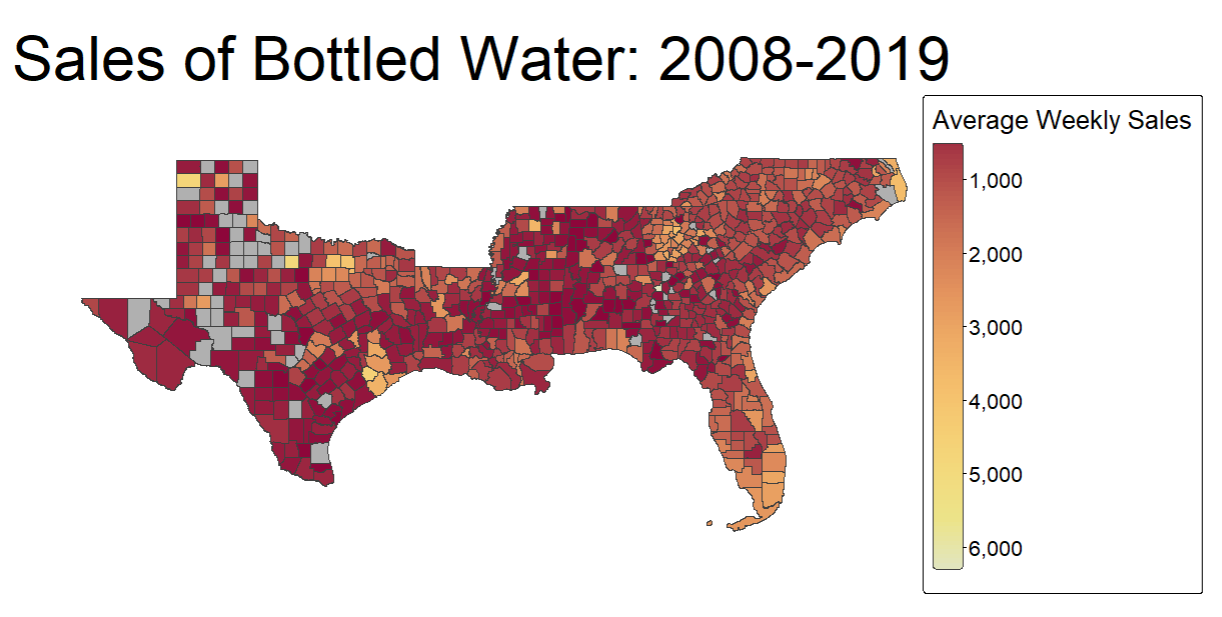
\includegraphics[width=0.75\linewidth]{images/total sales.png}
  \caption{Average Sales of Bottled Water}
  \floatfoot{Note: A map of the average total revenue from bottled water sales per store in each county from 2008 to 2019.}
\label{fig:sales}
\end{figure}

In order to understand average county-level responses to hurricanes, I aggregate the data to a county-week level. First I aggregate the sales of individual bottled water products in each store by calculating total revenue from and total volume\footnote{Volume is recorded in fluid ounces.} of bottled water sales and average price of all water sold. Then I combine the store level sales to the county by calculating the average total revenue per store, average total volume per store,  and the average price per store. The average weekly store revenue from bottled water sales for each county can be seen in figure~\ref{fig:sales}. 

\subsection{Hurricane Data}

When signs of a tropical system (potential hurricane) first appear, the National Oceanic and Atmospheric Administration (NOAA) begins tracking the system. NOAA gathers information on the size, wind speed, movement speed, ocean temperature, and other atmospheric conditions that will affect the tropical system. Using this information, they begin forecasting the system for the next 5 days. Specifically they forecast the expected wind speed and location along with potential storm surge, tropical storm watches and warnings, and hurricane watches and warnings \citep{NOAAforecast}. To keep the public well-informed on the formation and expected path of the system, NOAA posts a new forecast advisory every six hours. 

The National Hurricane Center (NHC) within NOAA houses extensive data sets on all current and past hurricanes. I utilize two of these data sets to build out variables on current and past hurricane activity. I build variables about hurricane forecasts and landfalls from 2008-2019 using the GIS Archive of Tropical Cyclone Forecasts. This archive contains all shapefiles used to build the hurricane forecasts and watch/warning advisories since the 2008 Atlantic Hurricane Season. The archive contains a new file for each advisory update, which occur every six hours from the system's formation to its dissipation. The files contain the geometries for the center track line, the forecast location of the hurricane at different times along the center track, and the cone-of-uncertainty around the center track.  Figure~\ref{fig:forecasts} shows the results of using the archived shape files to replicate the forecast as it was shared by NOAA in the past. 

\begin{figure}[t!]
   \centering
	\begin{subfigure}{0.45\linewidth}
		%\caption{Official Forecast}
		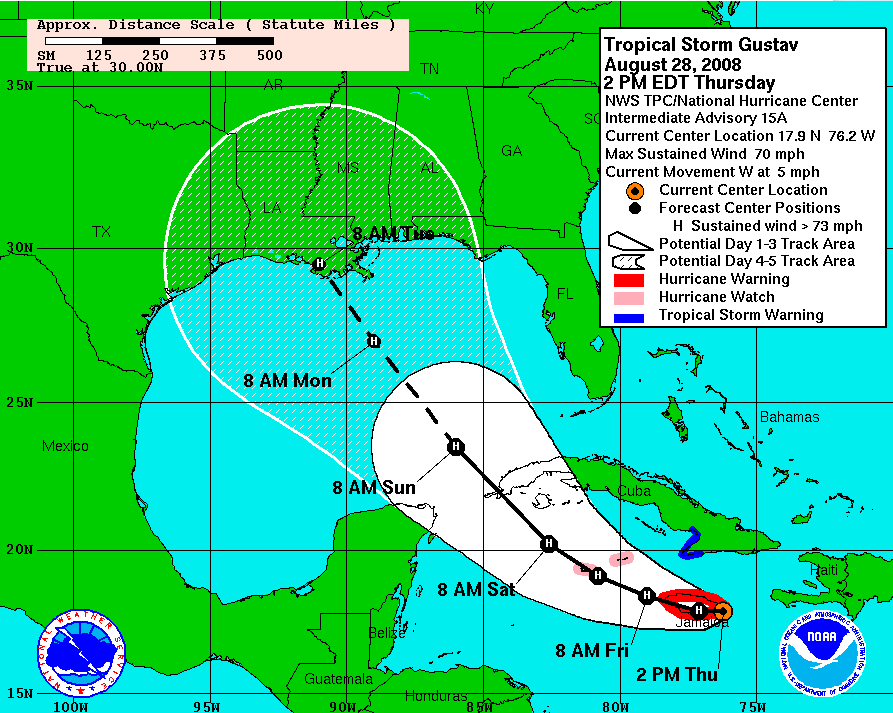
\includegraphics[width=\linewidth]{images/Gustav Official.png}
	\end{subfigure}
	\begin{subfigure}{0.45\linewidth}
		%\caption{Replication}
		\includegraphics[width=\linewidth]{images/forecast Rep.png}
	\end{subfigure}
  \caption{Replication of Official NOAA Forecast}
  \floatfoot{Note: Maps of official and replicated forecasts of Hurricane Gustav (2008). Official advisory (left) is from August 28, 2008, at 2pm with the replication (right) made from the archived shape file of the same advisory. Gustav made initial landfall in Louisiana at 10pm on Monday, September 1, 2008.}
\label{fig:forecasts}
\end{figure}

Using the archive I build out variables to indicate when a county is in the path of a hurricane, $Threatened$, and when a county is directly affected by a hurricane landfall, $Landfall$. To build out the $Threatened$ variable, I utilize the cone-of-uncertainty. If the county is within a cone-of-uncertainty at any point during the week of observation, it is classified as threatened. Because the cone-of-uncertainty is not actually showing where the entire hurricane may go, but rather where the center may go, I also define two additional threatened variables by buffering the cone-of-uncertainty at 50 and 100 nautical miles (NM)\footnote{NOAA measures distance in nautical miles and speed in knots. 50 and 100 nautical miles are respectively 57.5 and 115 miles and 92.6 and 185 kilometers.}.

I construct the $Landfall$ variable using the definition from the glossary of NHC terms: ``The intersection of the surface center of a tropical cyclone with a coastline'' \citep{NHCglossary}. I begin by mapping each recorded hurricane location and determining whether the hurricane center is over land or over water. Initial landfall occurs when the hurricane center moves from over water in one advisory to over land in the next advisory. For each point determined as an initial landfall, a circle is drawn around the point with a radius of 100NM. Any county that lies within this circle is considered to be affected by the landfall, and is indicated as such. Similar to $Threatened$, I draw additional circles to indicate landfall that extend the radius an additional 50 and 100NM. 

 \begin{figure}[t!]
   \centering
	\begin{subfigure}{0.7\linewidth}
		%\caption{Official NOAA Forecast August 28, 2008}
		\includegraphics[width=0.95\linewidth]{images/past landfall count.png}
	\end{subfigure}
	\begin{subfigure}{0.7\linewidth}
		%\caption{Replication from Archive of August 28, 2008}
		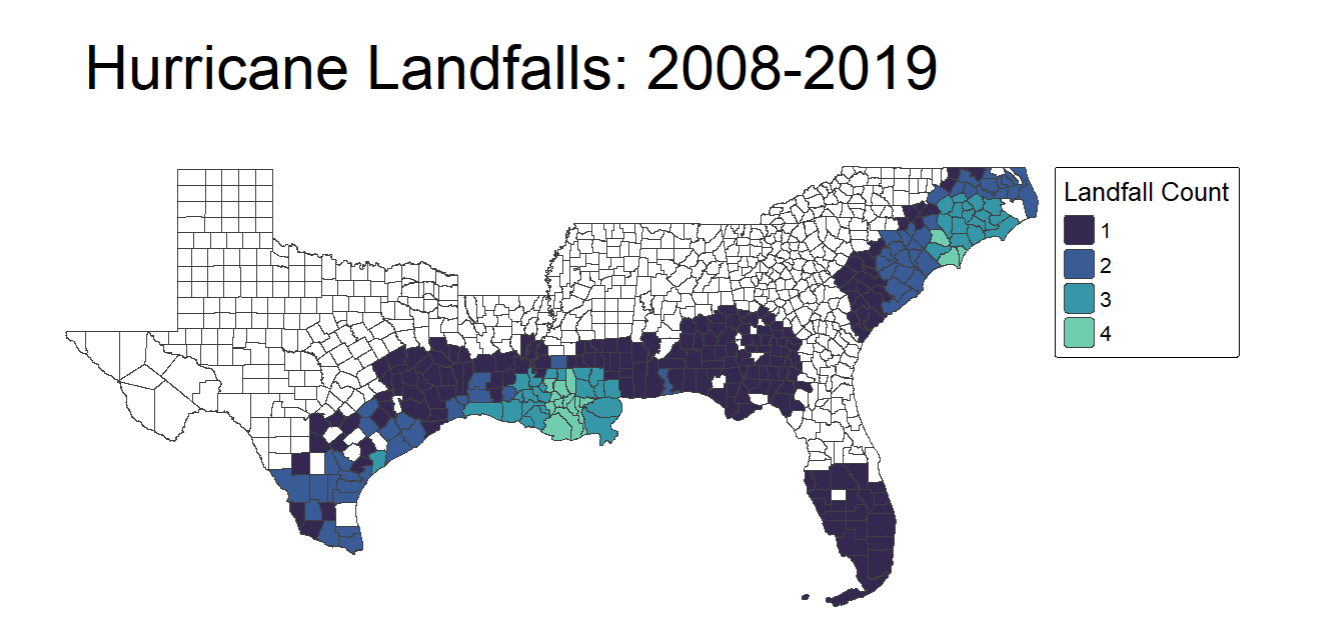
\includegraphics[width=\linewidth]{images/current landfall count.png}
	\end{subfigure}
  \caption{Total Hurricane Landfalls}
  \floatfoot{Note: Maps of total initial hurricane landfalls from 1983 to 2007 (top) and from 2008 to 2019 (bottom). The lighter colors represent more landfalls during the given time frame.}
\label{fig:hur_count}
\end{figure}


In addition to the GIS Archive, I also use \citeauthor{HURDAT2}'s HURDAT2, also known as the ``Best Track'' data set, to construct variables regarding each county's history with hurricanes. This data set contains the location and wind speed and an initial landfall indicator from each advisory of all recorded hurricanes as far back as the 1850s. Because hurricane tracking did not become consistent until more recently, I use the 25 years prior (1983--2007) to determine baseline historical variables. From this data, I create two variables to capture different aspects of a county's history with hurricanes. The first variable I create is the total hurricane landfalls in the last 25 years, $PastCount$. I create two versions of this variable, a static version based on the start of the data, and a continuous version that depends on the year in the data. 

I begin building the static version in a manner similar to the landfall variable above. For each past initial landfall in the HURDAT2 data, I draw a 100 nautical mile circle around its center and denote any counties within the circle. I then count the number of times each county appeared within a landfall circle in each of the past years. Finally I sum across years for each county to get the total number of landfalls in the 25 years before the scanner data began. To build the continuous version, I drop the oldest year of landfalls and add the most recent year so that in 2008 the past landfall count is from 1983--2007, and in 2009 the count is from 1984--2008. % add in table of summary stats, need to show that while there is enough variation to not lose to county fixed effects, it is not wild variation. 

Figure~\ref{fig:hur_count} shows the total count of hurricanes to make landfall in each county from 1983 to 2007 and from 2008 to 2019. It can be observed from these maps which specific regions of the Southeast are hotspots for hurricane landfalls. Interestingly, historical landfall counts do not perfectly correlate with the most recent decade of landfall. Specifically with parts of the Gulf Coast and South Florida only having 1 hurricane when they had been hit extensively before. This indicates that, while the overall patterns of hurricane landfall locations are not changing substantially, there is still meaningful variation in landfall exposure. 

\begin{figure}[t!]
   \centering
	\begin{subfigure}{0.7\linewidth}

		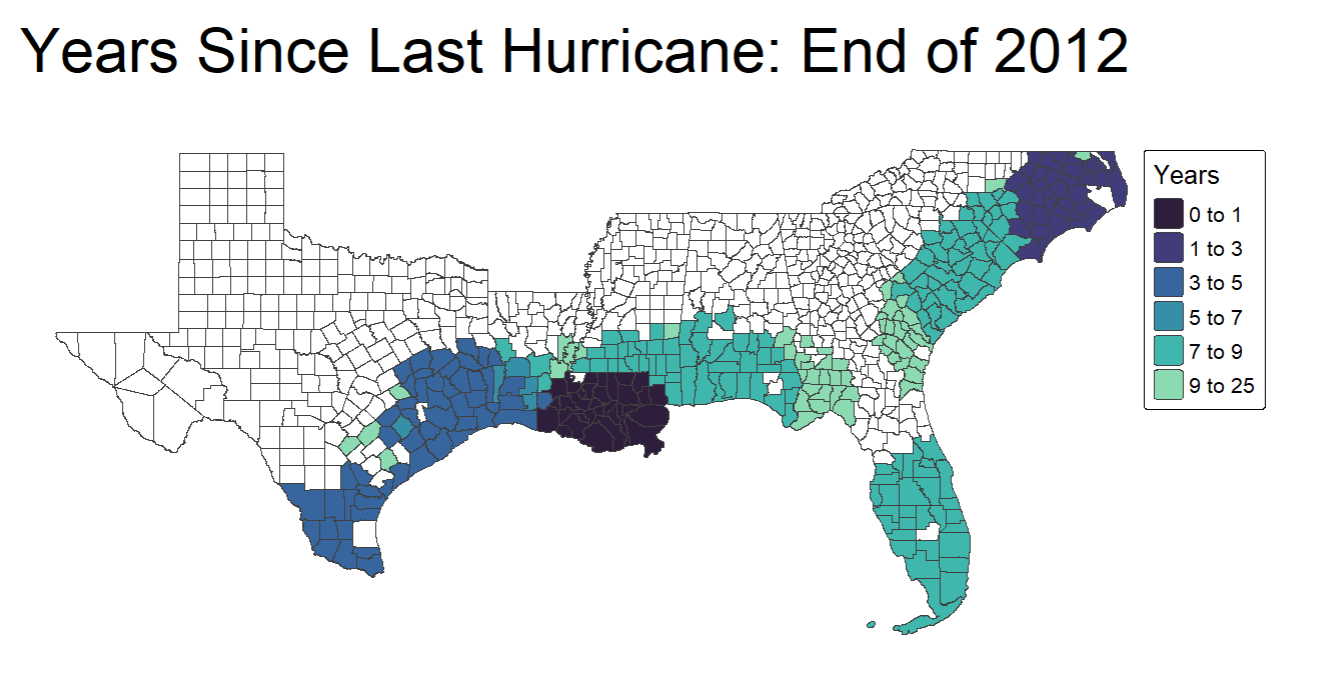
\includegraphics[width=\linewidth]{images/time 2012.png}
	\end{subfigure}
	\begin{subfigure}{0.7\linewidth}
		
		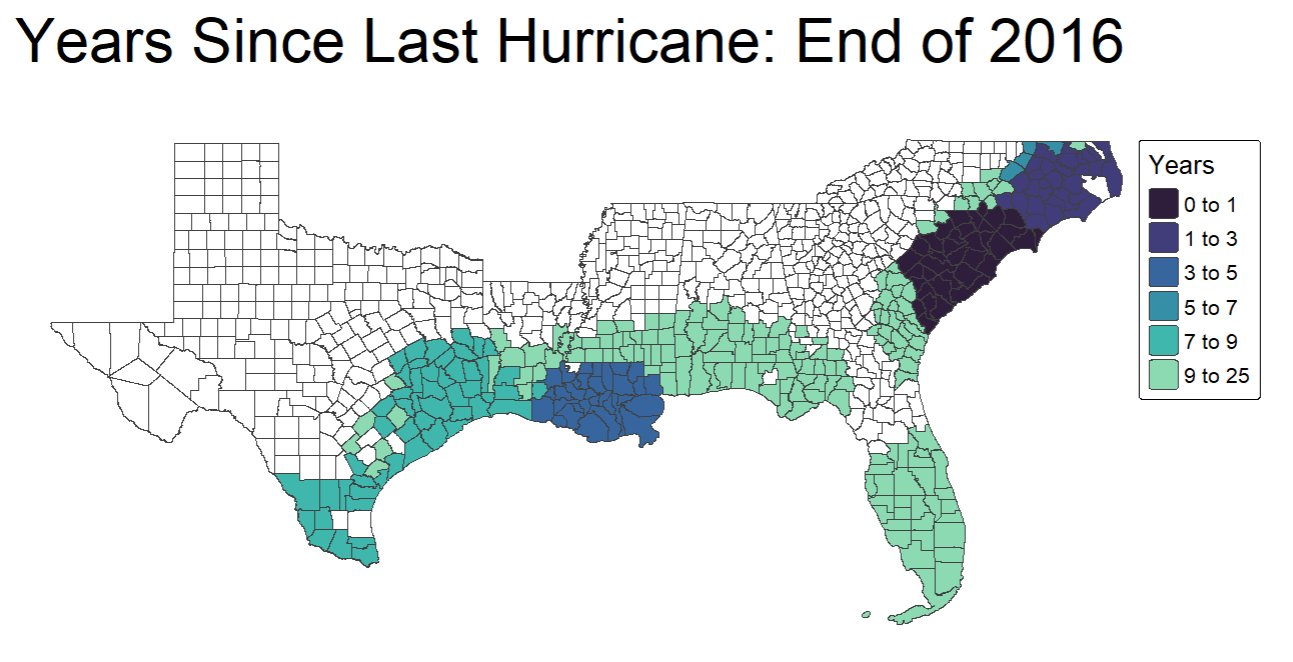
\includegraphics[width=\linewidth]{images/time 2016.png}
	\end{subfigure}
  \caption{Variation in Timing of Hurricane Landfalls}
  \floatfoot{Note: Maps representing the years that have passed since that last hurricane made landfall in a county. Each map is based on the hurricane record during the last week of the year. Thus, counties with 0 years since landfall in the top map were hit by a hurricane sometime in 2012. }
\label{fig:year between map}
\end{figure}

The second variable I create from this combined data is the length of time that passes between subsequent hurricane landfalls, $YearsSince$. While the landfall count gives us an idea of the average time between hurricanes, it is also possible for some counties to have repeat hurricanes rather quickly, and then not experience another hurricane for many years. One notable example is Palm Beach County, Florida which was hit by two hurricanes in both 2004 and 2005, was not hit again until 2016, and then experiences another hurricane in 2017. Using the HURDAT2 data, I find the latest date of landfall for each county. I begin my time between hurricane landfall variable in 2008 from this date. As counties experience new hurricane landfalls, the variable is reset to zero. The maps in figure \ref{fig:year between map} show the value for each county during the last week of the year in 2012 and 2016. Between these two years some counties experiences no additional hurricanes and therefore moved into longer-duration categories. Others experiences recent landfalls and moved into the shortest-duration category. Counties that appear in similar intermediate categories in both maps experiences landfalls between the two mapped years.


\subsection{Control Data}

To standardize the sales of bottled water, I pull in data from the \citeauthor{USCB}. Using the estimated county population measures from 2008 to 2019, I convert total revenue and total volume into totals per 100,000 residents. This transformation reduces the possibility that differences in county size or population changes mechanically drive the sales measures. After this transformation, cross-county variation in aggregate sales are substantially reduced, as shown in figure \ref{fig:per_cap_map} of the Appendix.   

Because bottled water sales may be affected by high heat days, I use data from \citeauthor{GHCN}'s Global Historical Climatology Network. Average temperature is recorded at the daily level at hundreds of weather stations across each state. I first match each county to its closest weather stations, then I take the average of the temperature across the entire week. Although weekly averaging smooths daily temperature variation, it captures whether a county-week was unusually hot and therefore more likely to have higher bottled-water demand unrelated to hurricanes. 

\section{Methodology}
% pick back up here

The empirical analysis estimates how bottled-water purchases respond to current hurricane threats and landfalls, and whether those responses differ with a county's hurricane history. The central empirical challenge is to distinguish the immediate effect of a current hurricane from differences in baseline purchasing patterns across counties with different levels of historical exposure. I therefore estimate models that compare sales within counties over time while controlling for common seasonal patterns, annual shocks, and local weather conditions.

The analysis proceeds in three steps. First, I estimate event-study models around hurricane landfalls to document the timing of bottled-water purchases before and after a current hurricane. Second, I estimate difference-in-differences models that test whether counties with greater historical hurricane exposure exhibit different baseline purchases or different storm-response purchases. Third, I estimate models that incorporate the time since the most recent hurricane landfall, conditional on historical exposure, to test whether responses weaken as hurricanes become less recent. This final specification is the primary test of whether repeated exposure is associated with complacency rather than stronger preparedness responses.

\subsection{Preliminary Analysis}

Before analyzing the effects of past county experiences on current purchases of bottled water, I first use a simple event study and regression model to test that there is observable changes in sales when there is a hurricane forecast in the likeness of \cite{beatty2019disaster}. 

\subsection{Historical Exposure and Storm Response Purchasing}

\subsection{Recency of Hurricane Experience}

\subsection{Robustness}

\subsection{Event Study Models}

I begin my analysis by conducting several event studies to test for more general impacts of county histories with hurricanes. The event studies are conducted using the following regression: 
\begin{equation}
Sales_{c,t} = \sum_{\tau = -10, \tau \neq -2}^{10} \beta_{\tau = t}L_{c,\tau = 0} + \alpha_c + \alpha_m + \alpha_y + \gamma X'_{c,t} + \varepsilon_{c,t}
\label{eq:ES}
\end{equation}
$Sales_{ct}$ represents the population-store weighted average total revenue from bottled water sales in a given county-week. The variable $L_{c, \tau = 0}$ indicates if a tropical system or hurricane makes landfall in a county during the event week $\tau = 0$. I use week $\tau = -2$ as the reference period for the event study to avoid spillover from the forecast in week $\tau = -1$. Because the scanner data is reported at a weekly level, if a storm were to make landfall early in week $\tau=0$ (i.e. Sunday or Monday), many of the purchases in advance would be done in the sales week before the storm lands, $\tau=-1$. The parameters of interest are $\beta_{\tau = -1}$, $\beta_{\tau = 0}$, and $\beta_{\tau = 1}$. Positive coefficients on $\tau = -1$ or $0$ would indicate that individuals are waiting for a storm to purchase emergency supplies. A null result on these weeks would indicate that there is little evidence to support the ``panic buying'' is a consistent behavioral response. Average weekly temperature is controlled for in $X'_{ct}$. County, month, and year fixed effects are represented as $\alpha_c$, $\alpha_m$, and $\alpha_y$ respectively. I allow for clustering of the standard errors at the county level.

To test for any effect from changes in total experience or from changes in timing between subsequent storms, I subset the data into quartiles along the $HurCount$ variable and again along the $YrSince$ variable. The quartiles for $HurCount$ are 1 to 7, 8 to 12, 13 to 16, and 17 or more. Because the variable is updated at the beginning of each year, it is possible for counties to move between quartiles or even pass counties that started in higher quartiles. Quartiles for $YrSince$ vary depending on how the variable is defined. When $YrSince$ is the number of years between the last storm of any kind and the next hurricane the quartiles are less than 1 year, 1 to 2 years, 3 years, and 4 or more years. When $YrSince$ looks exclusively at the years that pass between subsequent hurricanes, the quartiles are 1 to 2 years, 3 years, 4 to 6 years, and 7 or more years. Again, because the variable is continuously updating, counties may fall into multiple quartiles throughout the panel. 


% Section on incremental results. through regression interaction
\subsection{Interacted Regression Models}

After testing for quartile results with event studies, I move to regression analysis to test for incremental effects of experience with and timing between hurricanes. The model used in this portion of the analysis follows. 
\begin{equation}
\begin{split}
lnSales_{c,t} = &\beta_1 Threat_{c,t} + \beta_2 Landfall_{c,t} +\\ & \beta_3 H + \beta_4 H\times Threat_{c,t} + \beta_5 H\times Landfall_{c,t}+\\ &\alpha_c + \alpha_m + \alpha_y + \gamma X'_{c,t} + \varepsilon_{c,t}
\label{eq:gen_reg}
\end{split}
\end{equation}
The log of population-store weighted average total revenue from bottled water sales for a given county-week is represented by $lnSales_{c,t}$. $Threat$ indicates if a county was within the ``cone of uncertainty'' during any of the forecasts for that week. $Landfall$ indicates if a county was within the average landfall radius of a hurricane eye during the given week. The variable $H$ represents the historic hurricane related variables of interest, $HurCount$ and $YrSince$. Weekly temperature is controlled for in $X'$. Additionally, there are county level fixed effects, $\alpha_c$, as well as both year, $\alpha_y$, and month, $\alpha_m$ to capture any seasonality in sales. The variables of interest are $\beta_4$ and $\beta_5$ as these will indicate the effects of historical hurricane trends on ``panic buying'' related sales specifically. Standard errors are clustered by county-year. 

\subsection{Robustness}

Significant positive results of the coefficients from the linear model of years between are not inherently causal. Purchasing patterns could increase for a myriad of reasons beyond fading memory. Sales may also increase as years between subsequent hurricanes increases because people's purchasing changes to early in the hurricane season and then slowly changes back to a ``panic'' response. Sales could also increase because people have a stockpile from the prior hurricane that runs out over time, and the more time that passes, the more likely they are to need to restock. 

The first way to test for causality is to test if the change in response follows that of prior literature. Past literature on natural disasters and memory effects find a consistent result of an initial reaction followed by a dropoff in responsiveness \citep{gallagher2014learning,kelly2012evolution,MeyerEtAl14}. I test for changes in responsiveness in two ways. First, the event study model provides a visual test for any patterns in responsiveness. Second, I add a quadratic interaction in equation~\ref{eq:gen_reg} so that the new model is as follows.  
\begin{equation}
\begin{split}
lnSales_{c,t} = &\beta_1 Threat_{c,t} + \beta_2 Landfall_{c,t} + \beta_3 H + \\
&\beta_4 H\times Threat_{c,t} + \beta_5 H\times Landfall_{c,t}+\\
& \beta_6 H^2\times Threat_{c,t} + \beta_7 H^2\times Landfall_{c,t}+\\
 &\alpha_c + \alpha_m + \alpha_y + \gamma X'_{c,t} + \varepsilon_{c,t}
\end{split}
\label{eq:square}
\end{equation}
If the quadratic terms are significant, then it is more likely that this is a behavioral response rather than one of the other mechanisms driving the change. 

To further test for a causal relationship, I run the same event studies and regressions for the start of hurricane season (week containing June 1). Changes in sales during the start of the season would provide strong causal evidence that people are changing their behavior in response to the recentness of a hurricane. A lack of significant result at the start of the season indicate that it is likely some other cause.

Testing for current inventory holdings changes is beyond the scope of this paper. Because sales are only reported at a store-week level, it would not be possible to determine how much individual household level inventory changes. I analyze this effect using a different set of data in further research \citep{wood}.

% add 6 or more (Yes/no) test to robustness. 
% beginning of summer goes to robustness as well. 
% Filter out non hurricanes 

\section{Results}

\subsection{Event Study Results}
% Replication 

I begin my analysis by testing for aggregate effects of hurricane forecasts and landfalls. By running the event study from equation (\ref{eq:ES}) on all counties, I estimate the average response of all counties to a hurricane. Figure~\ref{fig:AGG_ES} Panel (a) shows a clear sudden increase in sales of bottled water during the weeks surrounding a hurricane landfall with sales increasing by over \$500. Sales more than two weeks before and after the hurricane are not significantly different from zero indicating the effect of the hurricane is temporary in nature and not permanent. These results follow closely to those of prior literature, namely~\cite{beatty2019disaster}.

\begin{figure}[t!]
	\centering
	\begin{subfigure}{0.45\linewidth}
		\caption{Bottled Water Sales}
		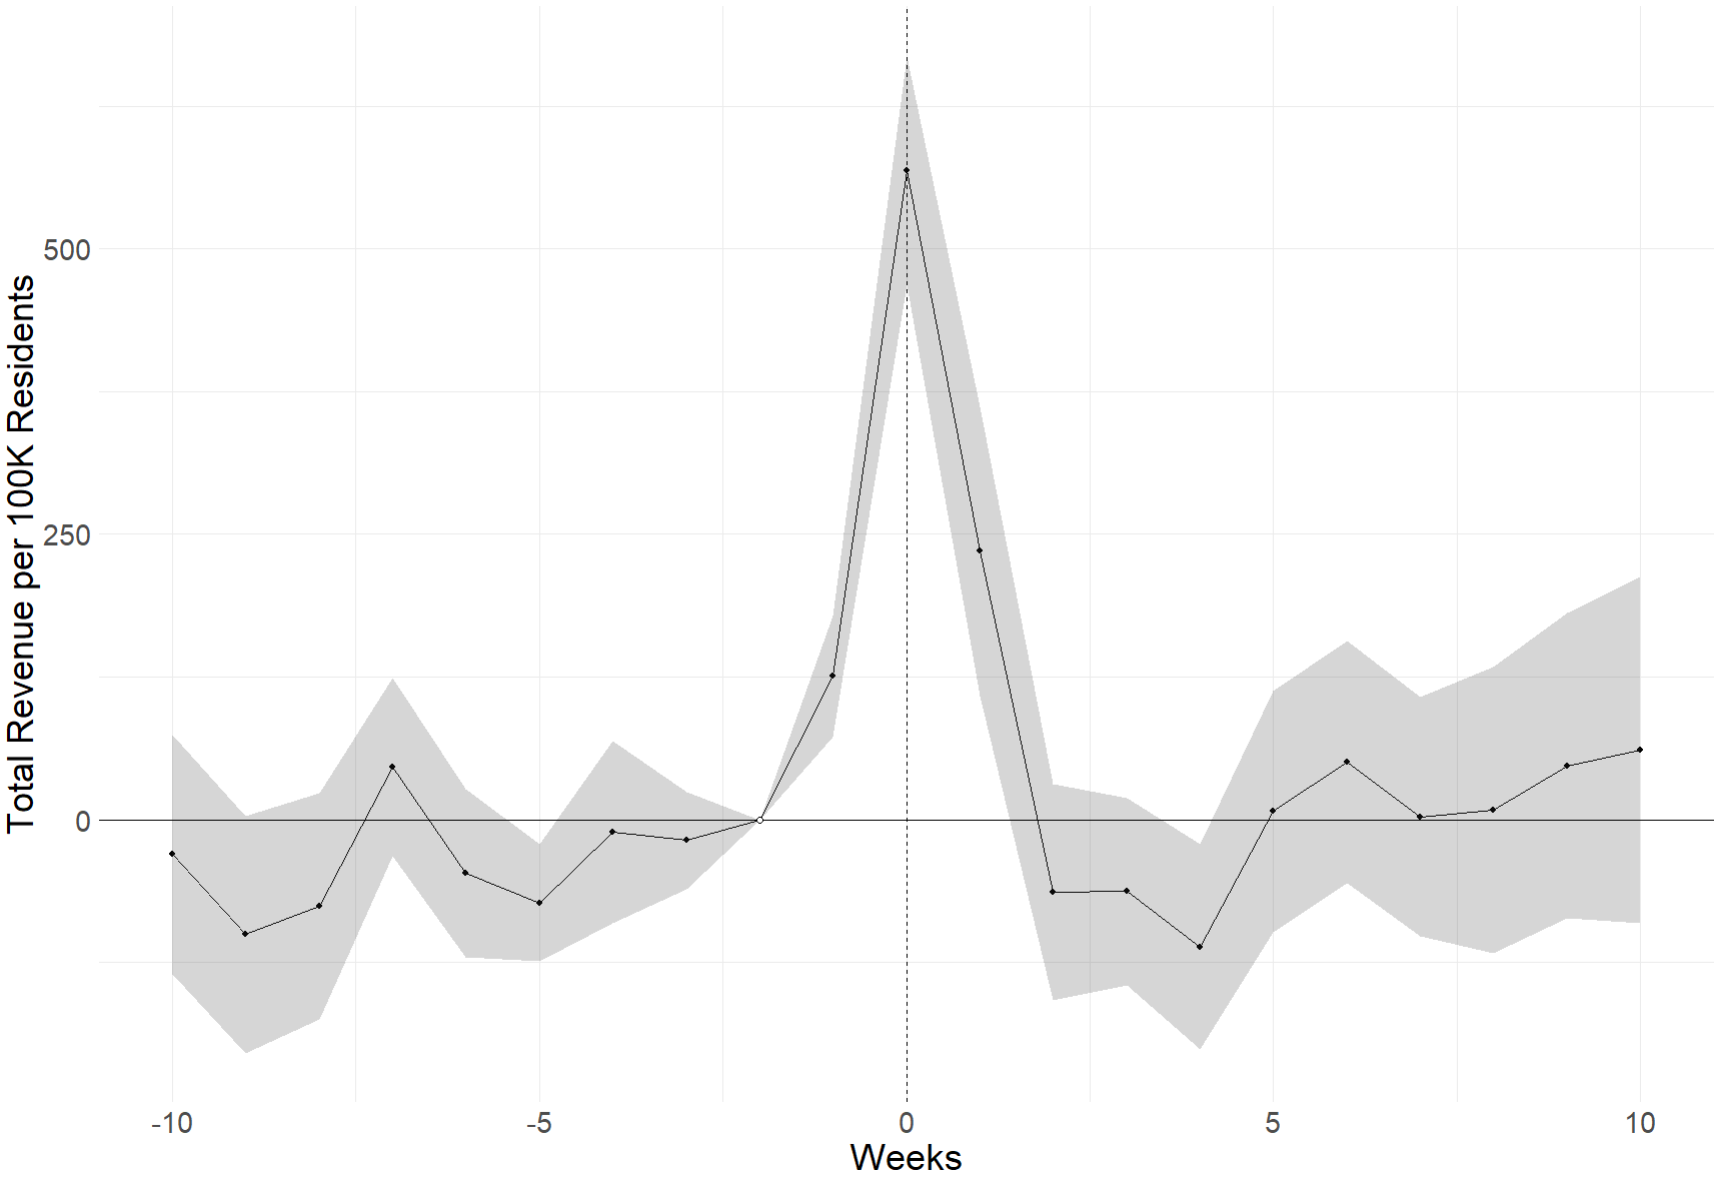
\includegraphics[width=\linewidth]{rev.png}
	\end{subfigure}
	\begin{subfigure}{0.45\linewidth}
		\caption{Price}
		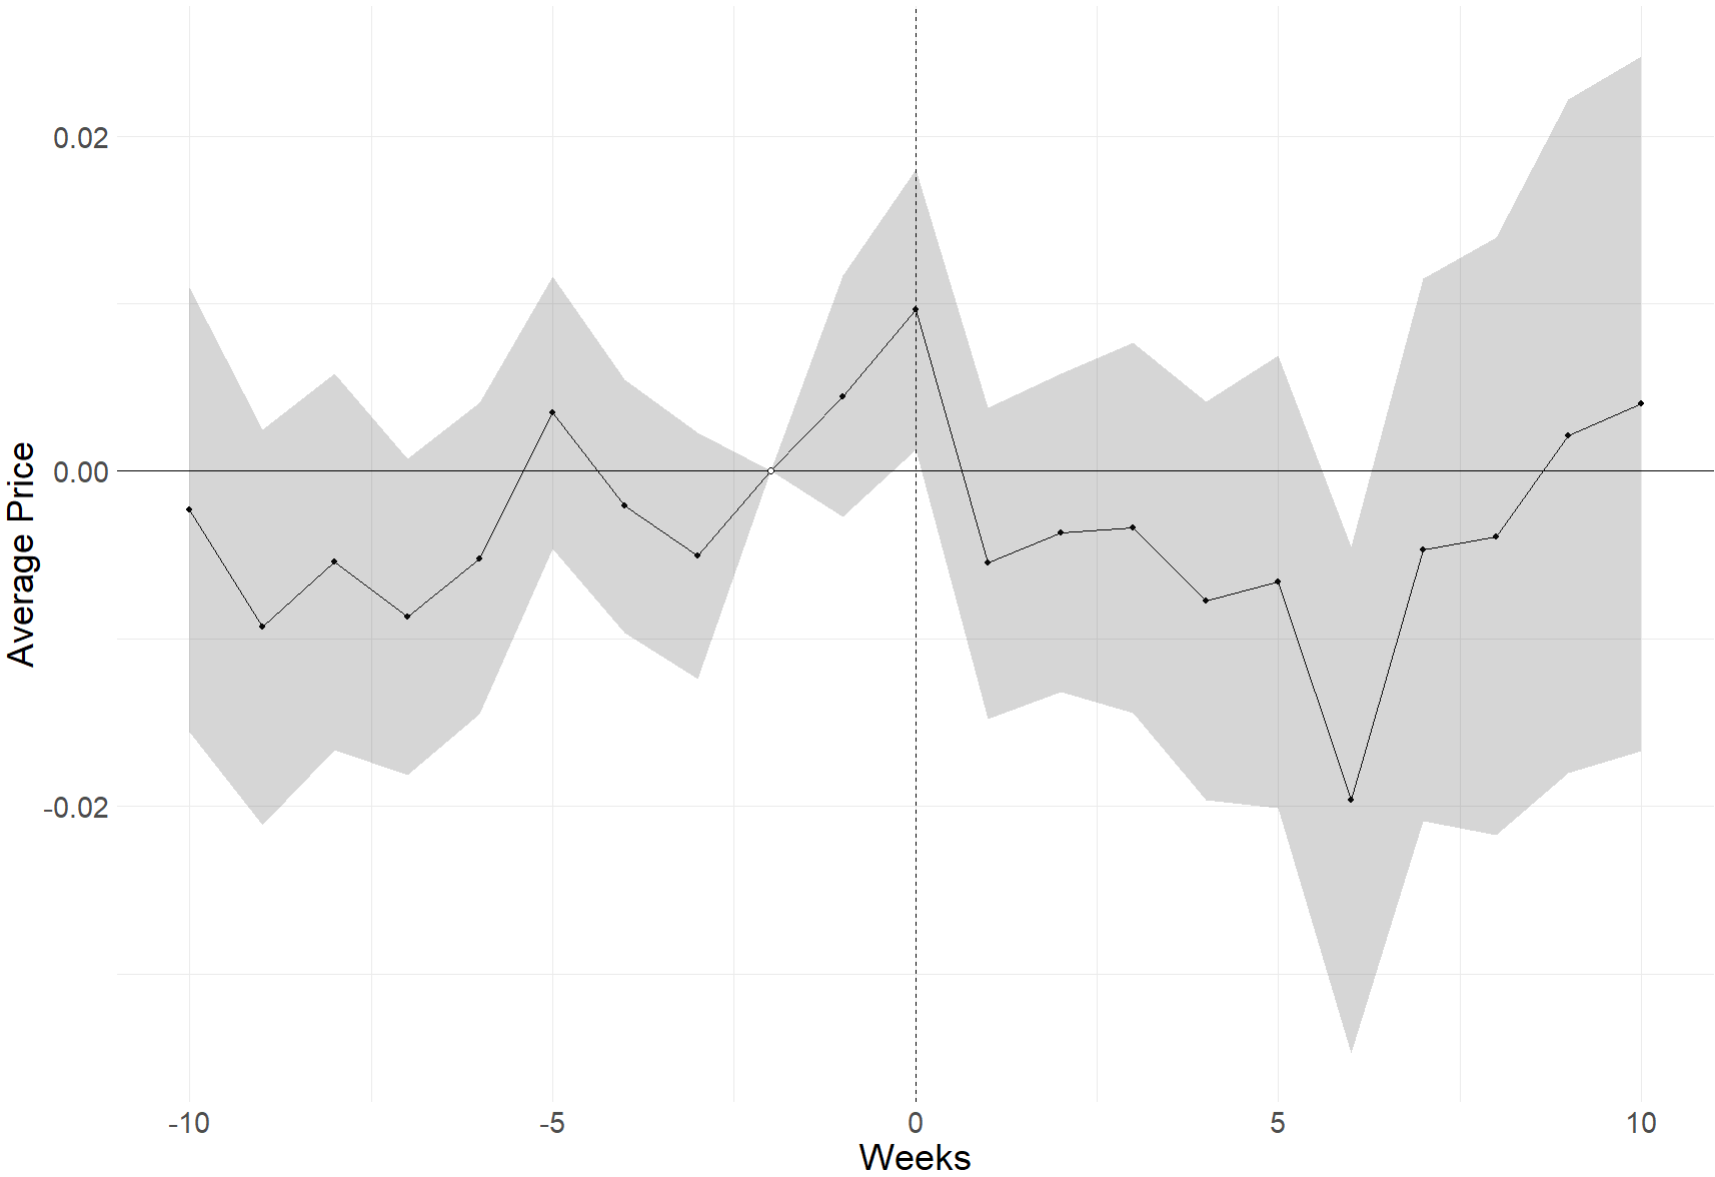
\includegraphics[width=\linewidth]{price.png}
	\end{subfigure}
	\caption{Aggregate Event Studies of Bottled Water Sales}
	\floatfoot{Note: Results from event studies following equation~\ref{eq:ES}. The vertical axis represents total revenue per 100 thousand residents in USD in panel (a) and average weekly price in panel (b). The horizontal axis represents weeks. The reference period is week -2. The vertical dashed line at week 0 represents the week when a storm made landfall. The ribbon around the estimates represents the 95\% confidence interval.}
	\label{fig:AGG_ES}	
\end{figure}

I also run the event study on the entire panel using price as the outcome variable rather than sales. Since the data is at a weekly level, price is the average price of bottled water in each county for the week. For any changes in sales responses to be behaviorally driven, it must come from a change in the amount that people are purchasing, not from changes in the pricing structure. Figure~\ref{fig:AGG_ES} panel (b) shows the results from the pricing event study. Here there are no significant changes in the price of bottled water, and the largest deviation seen during the hurricane is less than 1 cent. Thus, any changes in sales are likely from changes in consumer behavior.   

The HURDAT2 and GIS data include all classifications of tropical systems, yet news and social media sources tend to focus on systems classified as hurricanes and major hurricanes as these are the most destructive. I rerun the event study subdividing the data by three broad hurricane classification categories: less than hurricane, hurricane category 1--5, and major hurricanes (category 3--5). The results of the event study by category are in figure~\ref{fig:type}. It is clear from this figure that storms classified as a category 1 hurricane or stronger are driving all the results in Panel (a) of figure~\ref{fig:AGG_ES}. Confidence intervals can be seen in figure~\ref{fig:type_ci} in the appendix and show that the effects of hurricane and major hurricane landfalls are significantly different from the results from a landfall of a lesser system. Additionally, the effect of a lesser system are not significantly different from no storm at all. For the remainder of the analysis, I only look at the effects hurricane specific landfall.


\begin{figure}[t!]
    \centering
    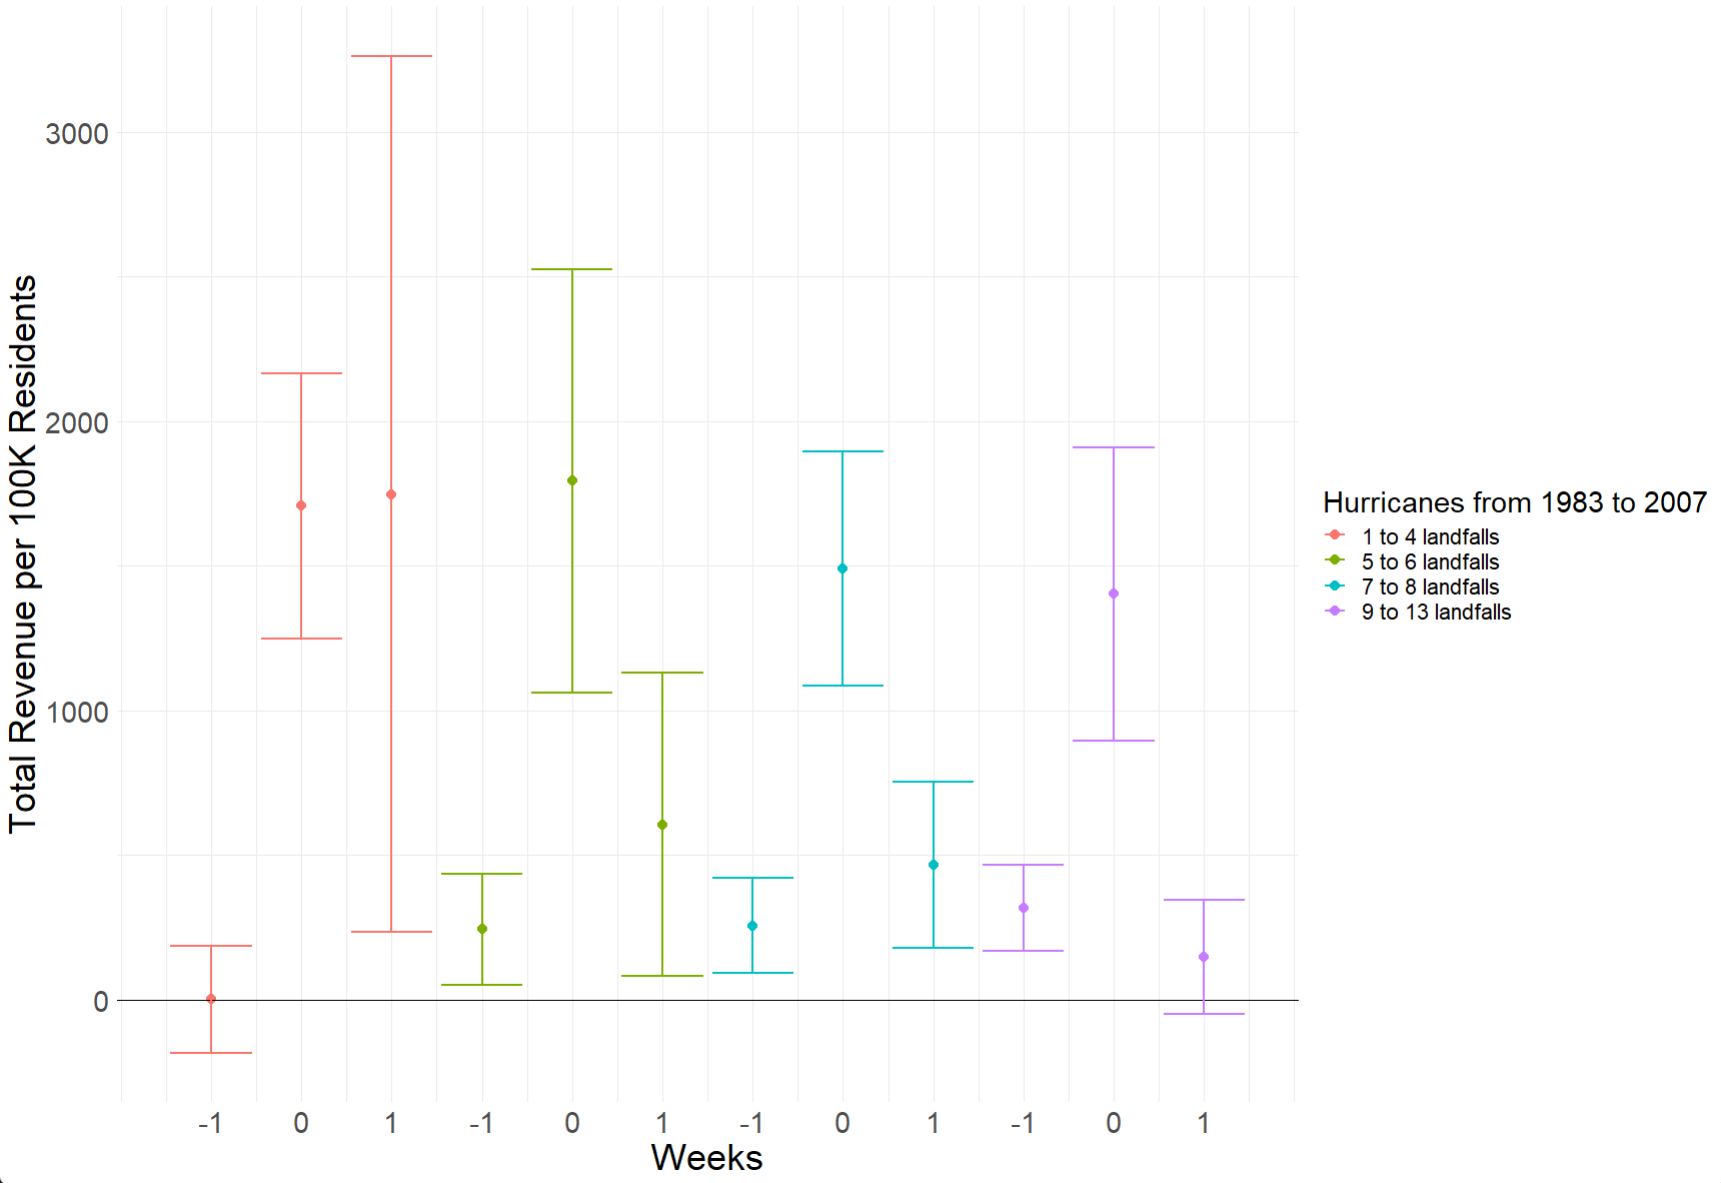
\includegraphics[width =0.9\linewidth]{hist quartiles.png}
    \caption{Event Studies of Historical Exposure on Sales}
    \label{fig:hist}
    \floatfoot{Note: Results from event study with subsets based on historical exposure of the county to hurricanes. The vertical axis represents total revenue per 100 thousand residents in USD. The horizontal axis represents weeks. Week 0 is the week that a tropical hurricane made landfall in a county. The bars represent the 95\% confidence interval around the point estimate.}
\end{figure}


I test for general effects of living in a more hurricane prone location by subsetting the data along the variable $HurCount$. The data is subset into the following quartiles: 1 to 7 prior landfalls, 8 to 12, 13 to 16, and 17 or more. Figure~\ref{fig:hist} shows the results of the event study along quartiles. The weeks shown in the graph are those immediately surrounding the hurricane landfall. Results of each full event study are show in appendix figure~\ref{fig:hist_full}. Consistent with the aggregate results, all quartiles respond significantly to a hurricane landfall, but the responses from one quartile to the next are not significantly different from one another. Additionally, the estimates on the week before landfall are not significantly different from one another. From this analysis alone, there is not enough evidence to support the argument that hurricane exposure directly increases knowledge. 


% Recency


I test for aggregate effects of repeated high intensity hurricane seasons by repeating the event study from equation (\ref{eq:ES}) with the panel subset by variable $YrSince$. The data is split into the following quartiles: 1 to 2 years between hurricanes, 3 year, 4 to 6 years, and 7 or more years. Figure~\ref{fig:disc} shows the results from this split of the data. The results seem to indicate a weak pattern of increased purchases as the number of years between subsequent years grows, eventually declining some time after year 6. The standard errors, however, are quite large resulting in estimates that are not significantly different from one another. 

\subsection{Regression Results}

While the event studies above fail to show any significant impact of both additional hurricane exposure and additional timing between hurricanes for broad categories, it is still possible that the incremental changes are significant. I continue my analysis by estimated fixed-effects regression model in equation~\ref{eq:gen_reg} for both additional hurricane landfalls, and additional years between subsequent hurricanes.

\begin{table}[htbp]
   \caption{Base Results}
   \centering
   \begin{tabular}{lccc}
      \tabularnewline \midrule \midrule
      Dependent Variable: & \multicolumn{3}{c}{Log Sales}\\
      Model:         & All Storms            & Hurricanes            & Hurricane Events\\  
      \midrule
      \emph{Variables}\\
      Threatened         & 0.0634$^{**}$  &  2.677$^{***}$              &   \\   
                     & (0.0266)       &   (0.0442)              &   \\   
      Landfall       & 0.1796$^{**}$  &      -2.060$^{***}$           &   \\   
                     & (0.0678)       &    (0.0446)            &   \\   
      Event          &                &                & 0.5645$^{***}$\\   
                     &                &                & (0.1143)\\   
      \midrule
      \emph{Fit statistics}\\
      Observations   & 448,123        & 448,123        & 448,123\\  
      R$^2$          & 0.77143        & 0.77155        & 0.77146\\  
      \midrule \midrule
      \floatfoot{Note: Column one runs the regression using all recorded systems. Column two using only systems that were classified as a category 1 hurricane or higher. Column three using systems category one and higher and combines Threatened and Landfall into one variable, Event. Log sales are the log total revenue from bottled water sales in U.S. dollars.  Mean weekly temperature is included as a control. standard errors reported in parentheses are clustered at the county-year level. Signif. Codes: ***: 0.01, **: 0.05, *: 0.1}
   \end{tabular}
\end{table}



\begin{table}[htbp]
   \caption{Historical Exposure Results}
   \centering
   \begin{tabular}{lccc}
      \tabularnewline \midrule \midrule
      Dependent Variable: & \multicolumn{3}{c}{Log Sales}\\
      Model:                             & (1)            & (2)            & (3)\\  
      \midrule
      \emph{Variables}\\
      Event                              & 0.5645$^{***}$ & 0.5371$^{***}$ & 0.5657$^{***}$\\   
                                         & (0.1143)       & (0.1150)       & (0.1755)\\   
      Past Count                    &                & -0.0868$^{**}$ & -0.0868$^{**}$\\   
                                         &                & (0.0369)       & (0.0369)\\   
      Event $\times$ Past Count     &                &                & -0.0057\\   
                                         &                &                & (0.0484)\\   
      \midrule
          \emph{Fit statistics}\\
      Observations                       & 448,123        & 448,123        & 448,123\\  
      R$^2$                              & 0.77146        & 0.77247        & 0.77247\\  
      \midrule \midrule
       \floatfoot{Note: Past Count is the total count of hurricanes for the 25 years before the current county-week observation. Log sales is the log total revenue from sales of bottled water in USD. Mean weekly temperature is included as a control. standard errors reported in parentheses are clustered at the county-year level. Signif. Codes: ***: 0.01, **: 0.05, *: 0.1}
   \end{tabular}
\end{table}

I start by estimating the effect of additional hurricane landfalls on sales. Table~\ref{tab:hist} shows the results from this specification. Column (1) shows the results of the base regression which excludes the historic county level variables. This column represents the average response of all counties. Although there is not a significant response to a hurricane threat, sales of bottled water increase by roughly 56\% when there is a hurricane landfall. 

Column (2) shows the results from adding total hurricane landfalls since 1980 to the regression. It is clear that total exposure to hurricanes significantly affect not only the scale of purchases, but also the timing of such purchases. As a county experience additional hurricanes, sales shift to earlier in the forecast process. Specifically, there is a 6\% decrease in sales associated with landfall, that are balanced by an equal 6\% increase in sales from threats. While the event study results in figure~\ref{fig:hist} were week, they do visually follow this pattern of an increase in sales before a hurricane and a decrease in sales during the hurricane week. 

% Rerun with looking at ts only, hur only, major hur only. See if get stronger results with more specificity.

\begin{table}[htbp]
   \caption{Recent Exposure Results}
   \centering
   \begin{tabular}{lcccc}
      \tabularnewline \midrule \midrule
      Dependent Variable: & \multicolumn{4}{c}{Log Sales)}\\
      Model:                                                                & (1)            & (2)            & (3)            & (4)\\  
      \midrule
      \emph{Variables}\\
      Event                                                                 & 0.5645$^{***}$ & 0.5291$^{***}$ & 0.6481$^{***}$ & 0.5207\\   
                                                                            & (0.1143)       & (0.1164)       & (0.1444)       & (0.4161)\\   
        Past Count                                                       &                & -0.0869$^{**}$ & -0.0869$^{**}$ & -0.0868$^{**}$\\   
                                                                            &                & (0.0345)       & (0.0345)       & (0.0350)\\   
      Years Since                                                &                & 0.0145$^{**}$  & 0.0146$^{**}$  & 0.0152$^{*}$\\   
                                                                            &                & (0.0065)       & (0.0065)       & (0.0082)\\   
      Event $\times$ Years Since                                 &                &                & -0.0156        & 0.0153\\   
                                                                            &                &                & (0.0089)       & (0.0205)\\   
      Event $\times$ Past Count                                        &                &                &                & 0.0489\\   
                                                                            &                &                &                & (0.0416)\\   
      Past Count$\times$ Years Since                       &                &                &                & -0.0002\\   
                                                                            &                &                &                & (0.0015)\\   
      Event $\times$ Past Count $\times$ Years Since        &                &                &                & -0.0115$^{*}$\\   
                                                                            &                &                &                & (0.0058)\\   
      \midrule
      \emph{Fit statistics}\\
      Observations                                                          & 448,123        & 190,566        & 190,566        & 190,566\\  
      R$^2$                                                                 & 0.77146        & 0.79132        & 0.79134        & 0.79141\\  
      \midrule \midrule
         \floatfoot{Note: Past Count is the total count of hurricanes for the 25 years before the current county-week observation. Log sales is the log total revenue from sales of bottled water in USD. Mean weekly temperature is included as a control. standard errors reported in parentheses are clustered at the county-year level. Signif. Codes: ***: 0.01, **: 0.05, *: 0.1}
   \end{tabular}
\end{table}

Next, I analyze the effect of additional years between subsequent hurricanes. Table~\ref{tab:years} shows the results from both equations~\ref{eq:gen_reg} and~\ref{eq:square}. In addition to controlling for temperature in these regressions, I also control for the total historical landfalls from above. The result is a significant decrease in early sales by roughly 13\% with an equal increase in sales closer to landfall. This is consistent with the results observed in the event study, and with the notion of fading memory. 

% also need to run one that does a 7+ cutoff.

\subsection{Robustness}

I test for the quadratic relationship of years between subsequent hurricanes and sales using the model in equation~\ref{eq:square}. Table~\ref{tab:years} column (3) shows the results from this specification. Adding the squared term affects the baseline holdings of water, but does not affect the sales during a hurricane forecast or landfall.

% need placebo regressions
% Show to ES also broken out by quartiles. This proves that no groups are balancing each other out by behaving oppositely.

% Because of anti-price gouging laws implemented by states during natural disasters, it is possible that prices are not allowed to move as they normally would from week to week. To ensure that government intervention is not biasing the results I rerun the analysis above using volume rather than revenue. For bottled water I use gallons, and for batteries and flashlights I use individual items (this is items in a pack so a pack of four batteries is four). Results for both the event studies and regression are nearly identical as when I use total revenue indicating that the results are being entirely driven by the consumers. The graphs and tables for these results can be found in section B of the appendi

\section{Conclusion}

As climate change continues, the intensity of natural disasters and extent of their destruction are expected to increase. Because this destruction also inhibits relief efforts, it is crucial that people know how to prepare for such disasters so that this delay is not harmful. I find that as counties are exposed to more hurricanes, the sales of emergency supplies actually increase in the presence of a storm. This indicates that people in these counties are learning how to prepare for disasters and adjusting. Additionally, the sales of emergency supplies decline in a way that follows the pattern of risk salience that is seen in other parts of the natural disaster literature when people are faced with a recurring disaster. The combination of needing experience and recent storms to purchase larger quantities of emergency supplies could leave areas with less experience or without a recent storm unprepared when faced with a hurricane. To help reduce the strain on relief efforts during future disasters, it be useful to find ways to bridge these gaps in emergency purchases.




\newpage
 \bibliographystyle{apalike}
 \bibliography{biblio}
\newpage



\begin{appendices}
\section*{Appendix}
\setcounter{table}{0}
\setcounter{figure}{0}
\renewcommand{\thetable}{A\arabic{table}}
\renewcommand{\thefigure}{A\arabic{figure}}


\begin{figure}[h!]
    \centering
    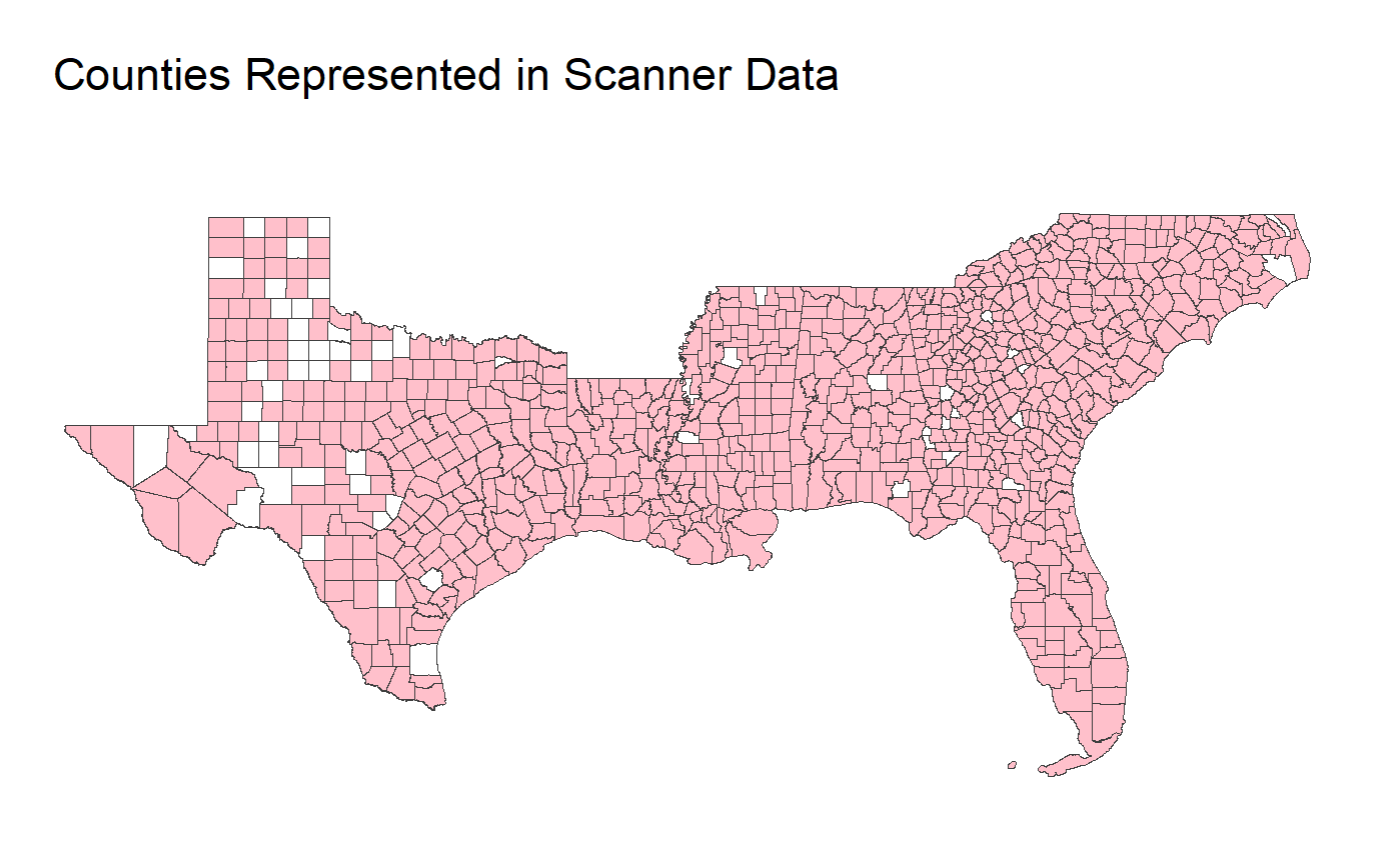
\includegraphics[width =0.8\linewidth]{scanner map.png}
    \caption{Counties Represented in Scanner Data}
    \label{fig:county_rep}
    \floatfoot{Note: A map of all counties that are represented in the scanner data. Represented counties have at least one store that reports to NielsenIQ. Unshaded counties do not have any reporting stores and so do not appear in the data. }
\end{figure}


\begin{figure}[h!]
    \centering
    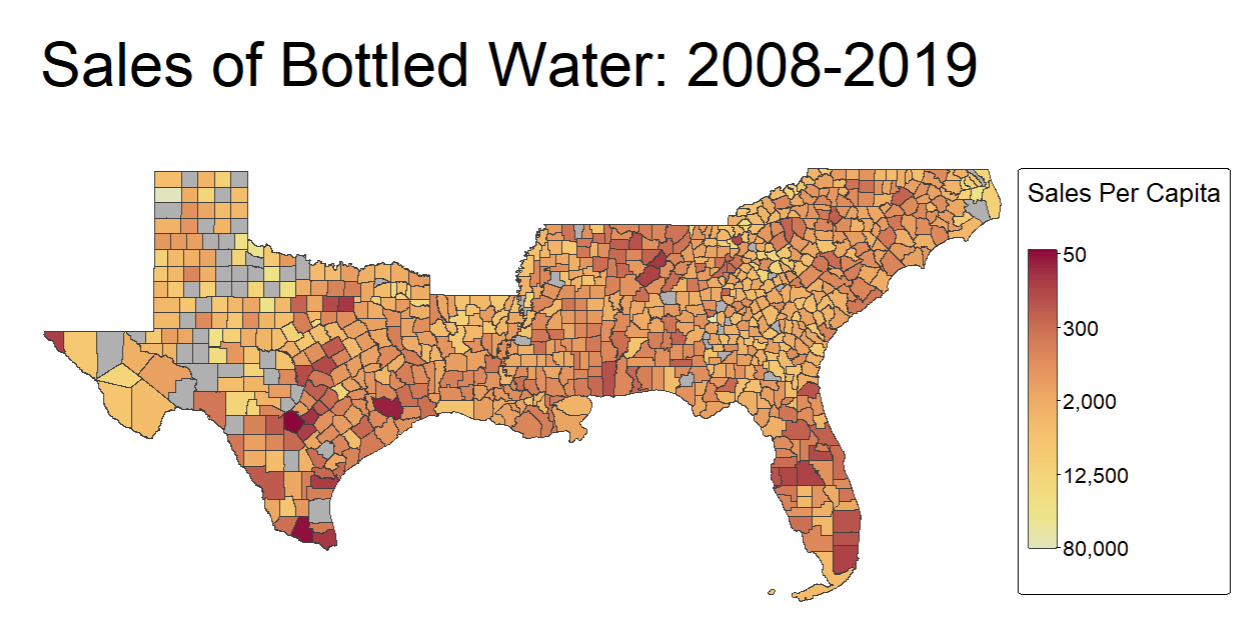
\includegraphics[width =0.8\linewidth]{per cap sales.png}
    \caption{Weekly Sales Per 100,000 Residents}
    \label{fig:per_cap_map}
    \floatfoot{Note: Total revenue in USD per 100,000 residents by county. Population measures are from the 2010 U.S. Census. Counties in grey are not represented in the NielsenIQ data.  }
\end{figure}


\begin{figure}[h!]
    \centering
    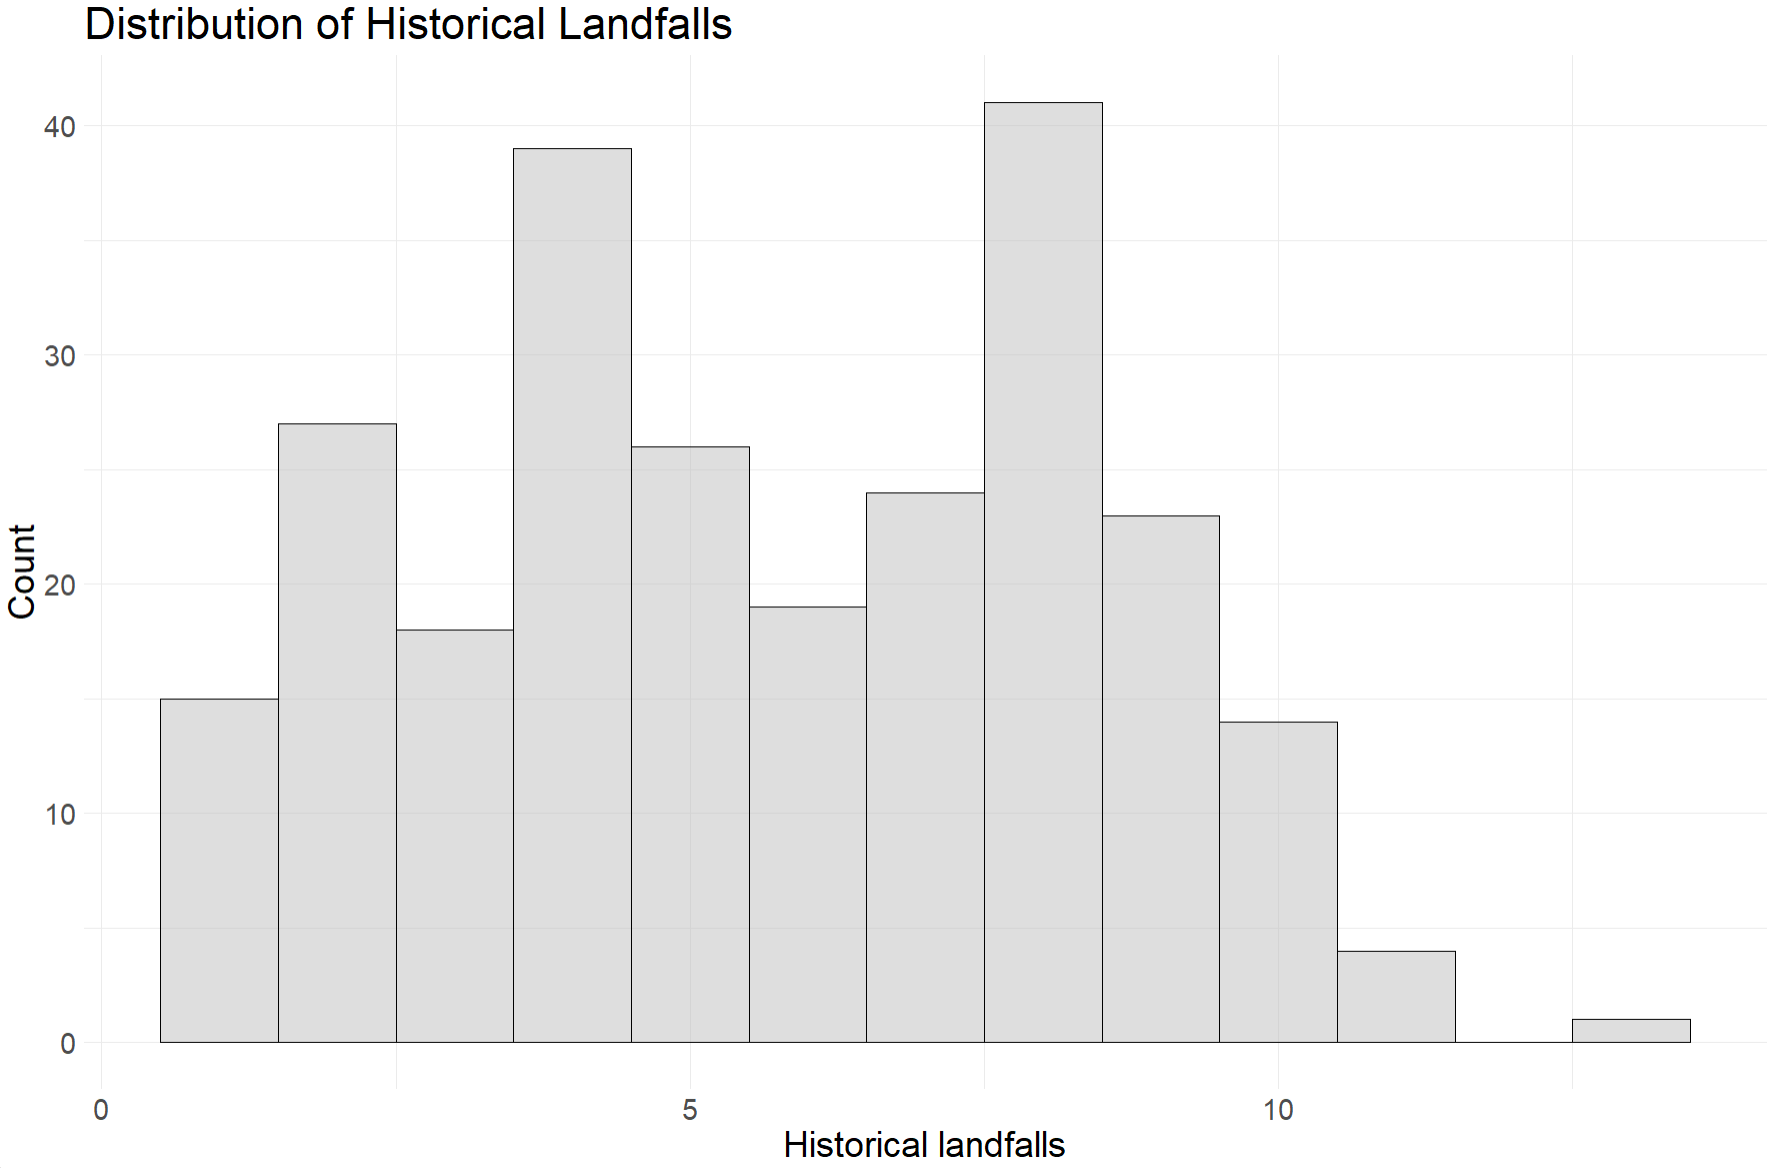
\includegraphics[width =0.65\linewidth]{hist hur dist.png}
    \caption{Histogram of Hurricane Landfall Counts}
    \label{fig:hist_total}
    \floatfoot{Note: The distribution of total hurricane landfall count from 1983 to 2007. Each observation is one county. }
\end{figure}

\begin{figure}[h!]
    \centering
    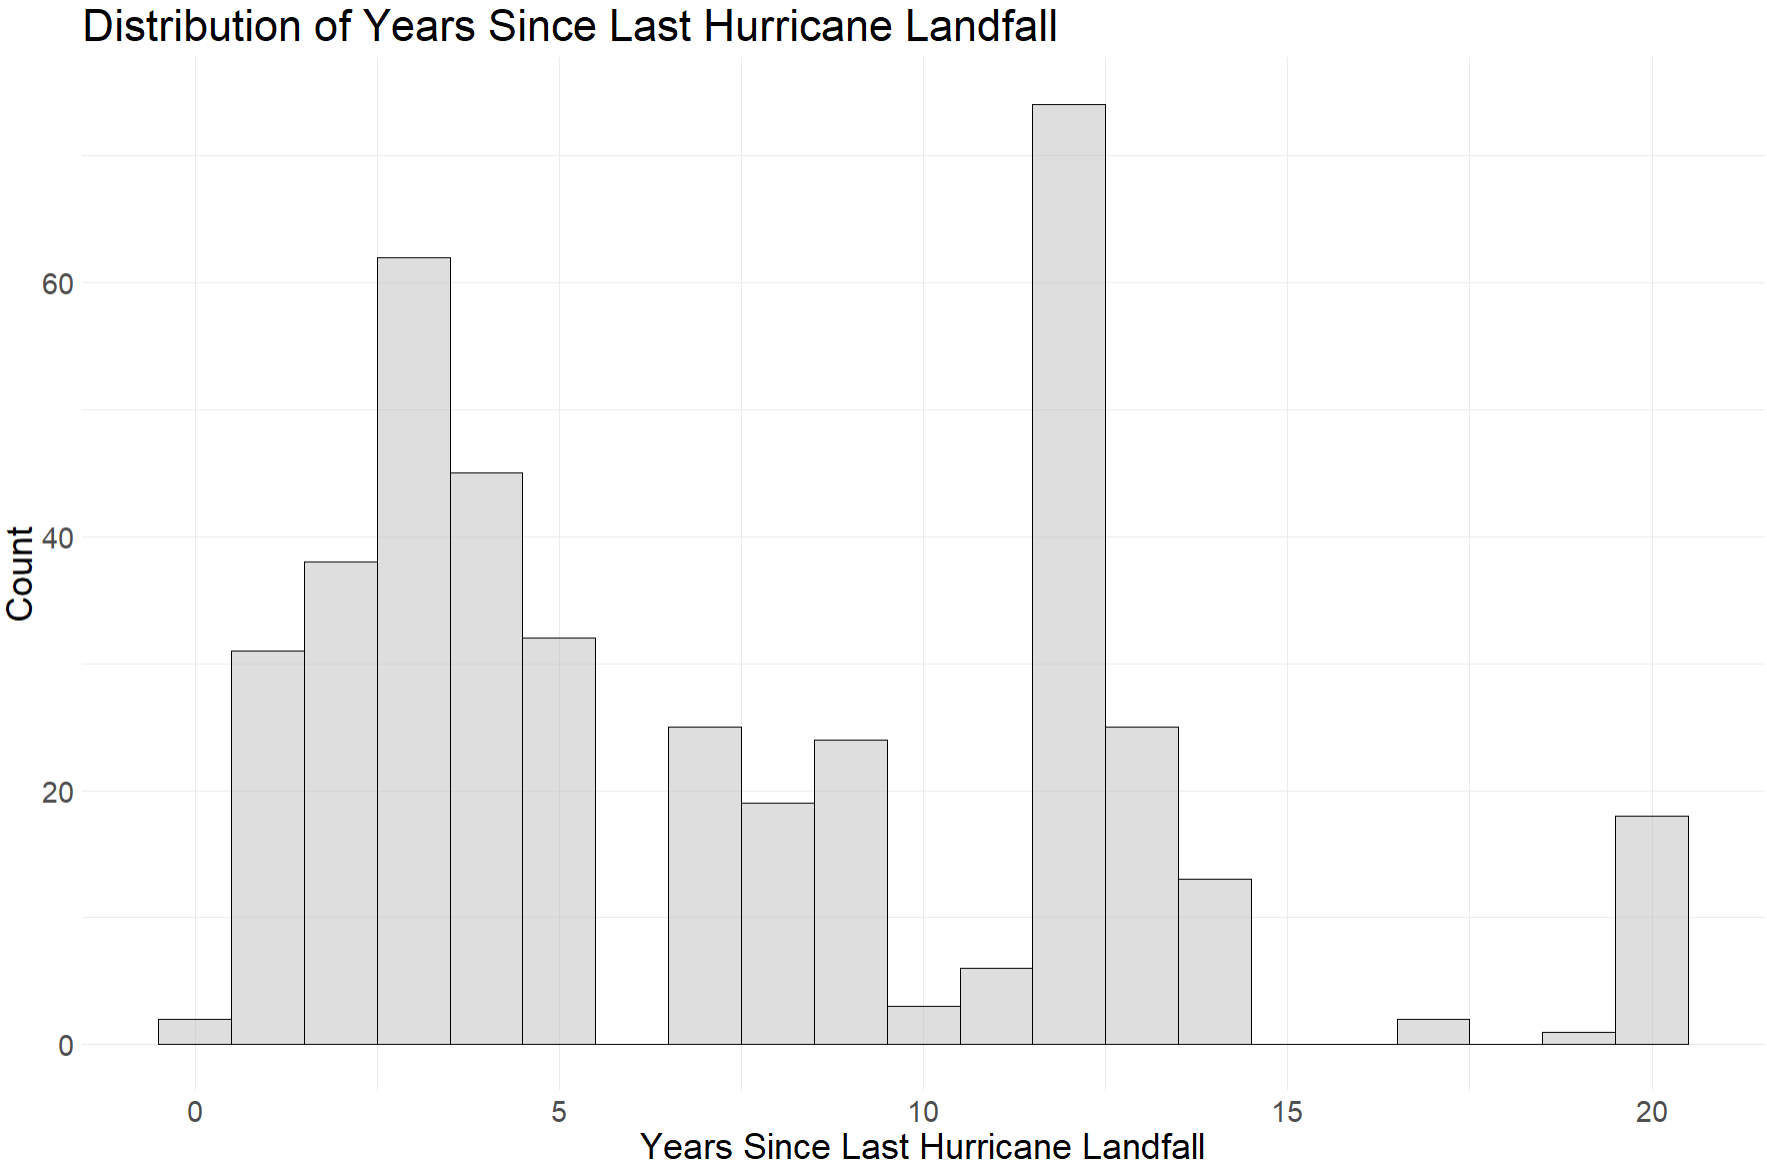
\includegraphics[width =0.65\linewidth]{time dist.png}
    \caption{Histogram of Years Between Hurricanes}
    \label{fig:hist_time}
    \floatfoot{Note: The distribution of time since the most recent hurricane for all county-hurricane landfalls from 2008-2019. Each observation is one county-hurricane instance.}
\end{figure}

\begin{figure}[h!]
    \centering
    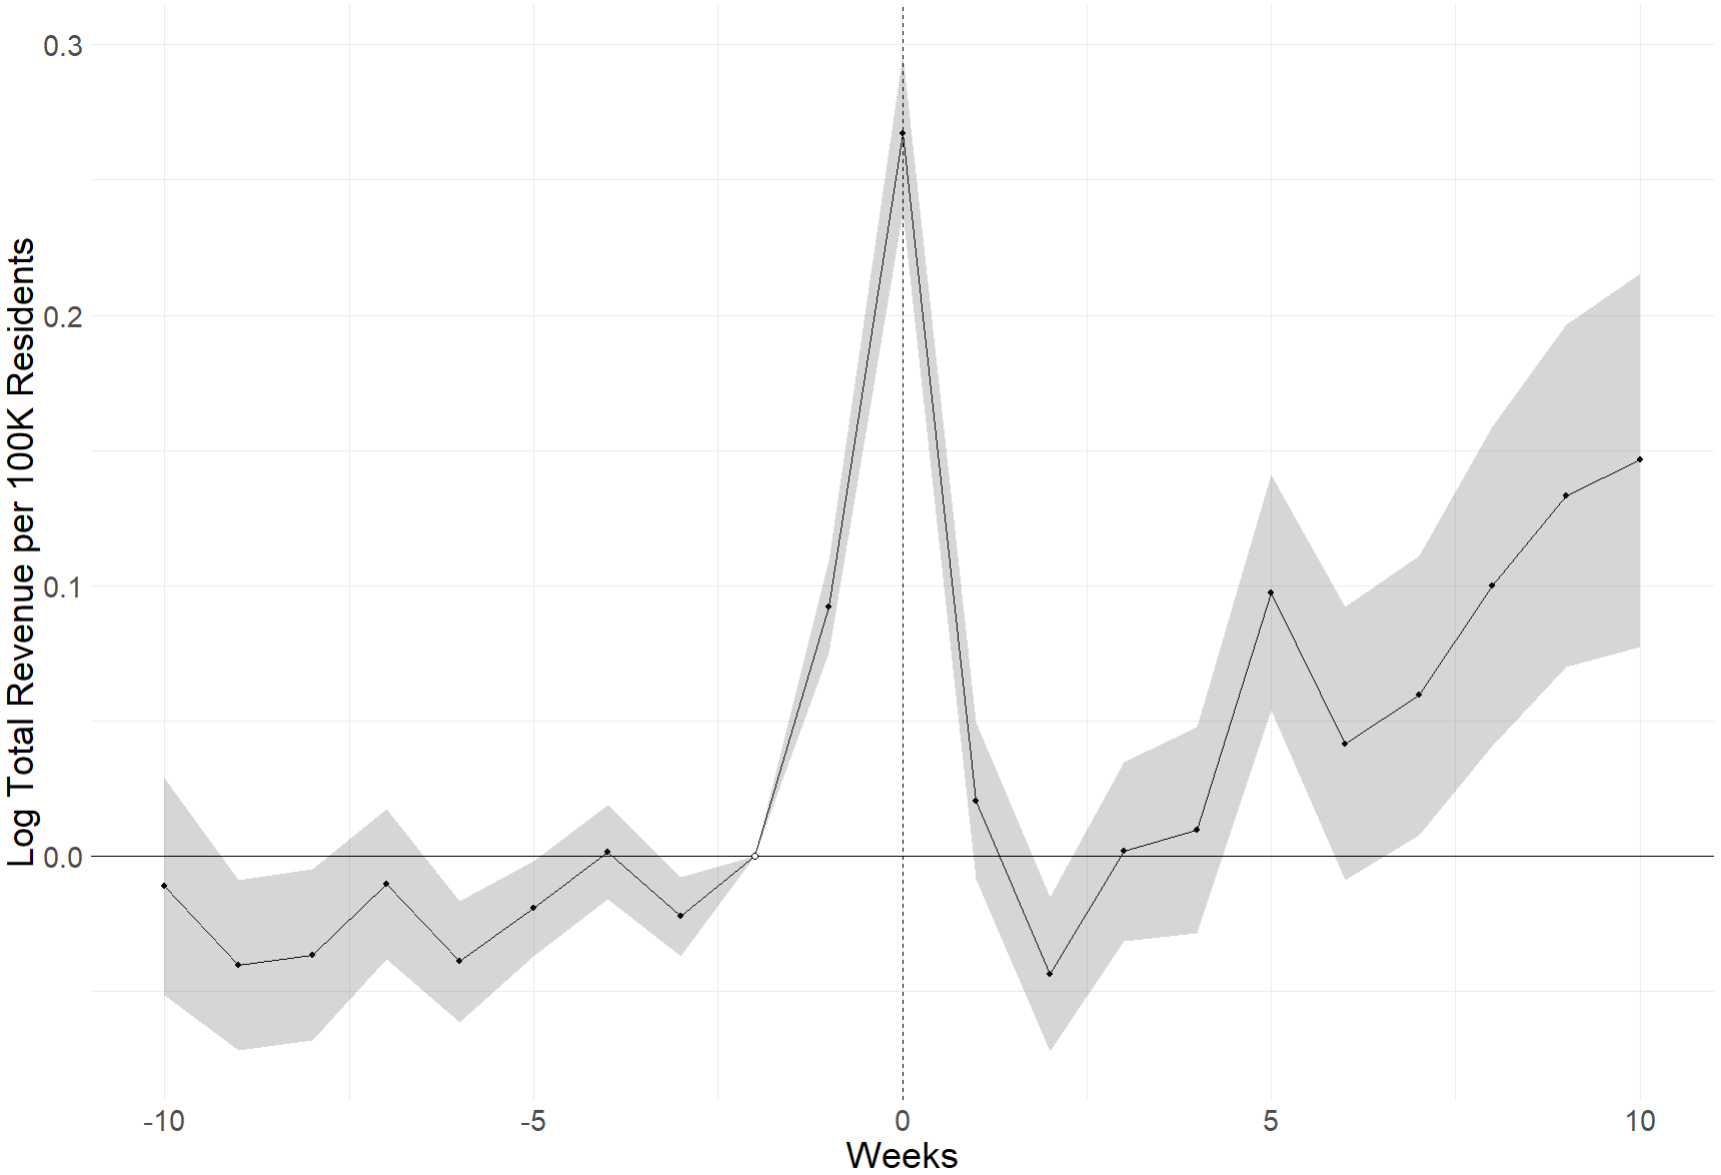
\includegraphics[width =0.7\linewidth]{log rev.png}
    \caption{Event Studies of Log Total Revenue}
    \label{fig:ES_log_rev}
    \floatfoot{Note: Results from event study with subsets based on hurricane category. The vertical axis represents natural log of total revenue from sales of bottled water in a county. The horizontal axis represents weeks. Week 0 is the week that a tropical hurricane made landfall in a county. The ribbon around each point represents the 95\% confidence interval.}
\end{figure}


\begin{figure}[h!]
    \centering
    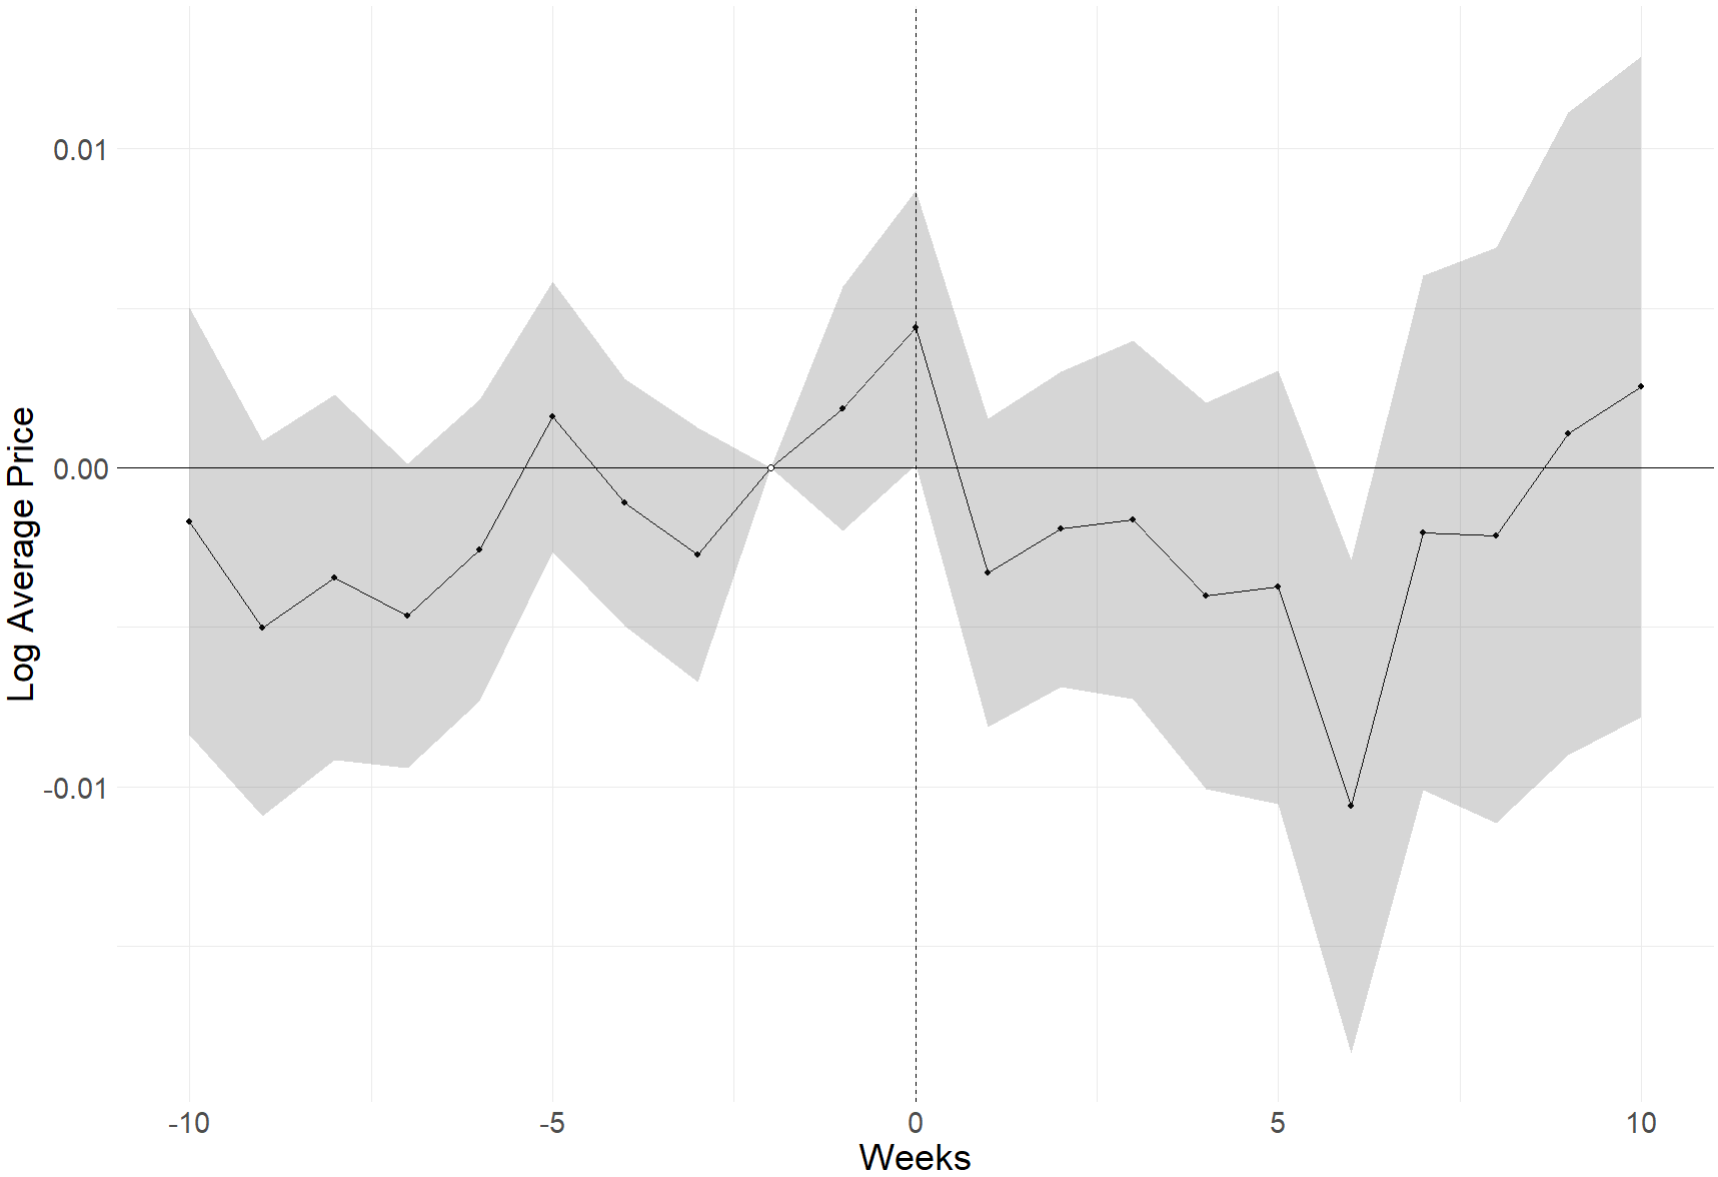
\includegraphics[width =0.7\linewidth]{log price.png}
    \caption{Event Studies of Log Price}
    \label{fig:ES_log_price}
    \floatfoot{Note: Results from event study with subsets based on hurricane category. The vertical axis represents log average price of bottled water in a county. The horizontal axis represents weeks. Week 0 is the week that a tropical hurricane made landfall in a county. The ribbon around each point represents the 95\% confidence interval.}
\end{figure}



\begin{figure}[h!]
    \centering
    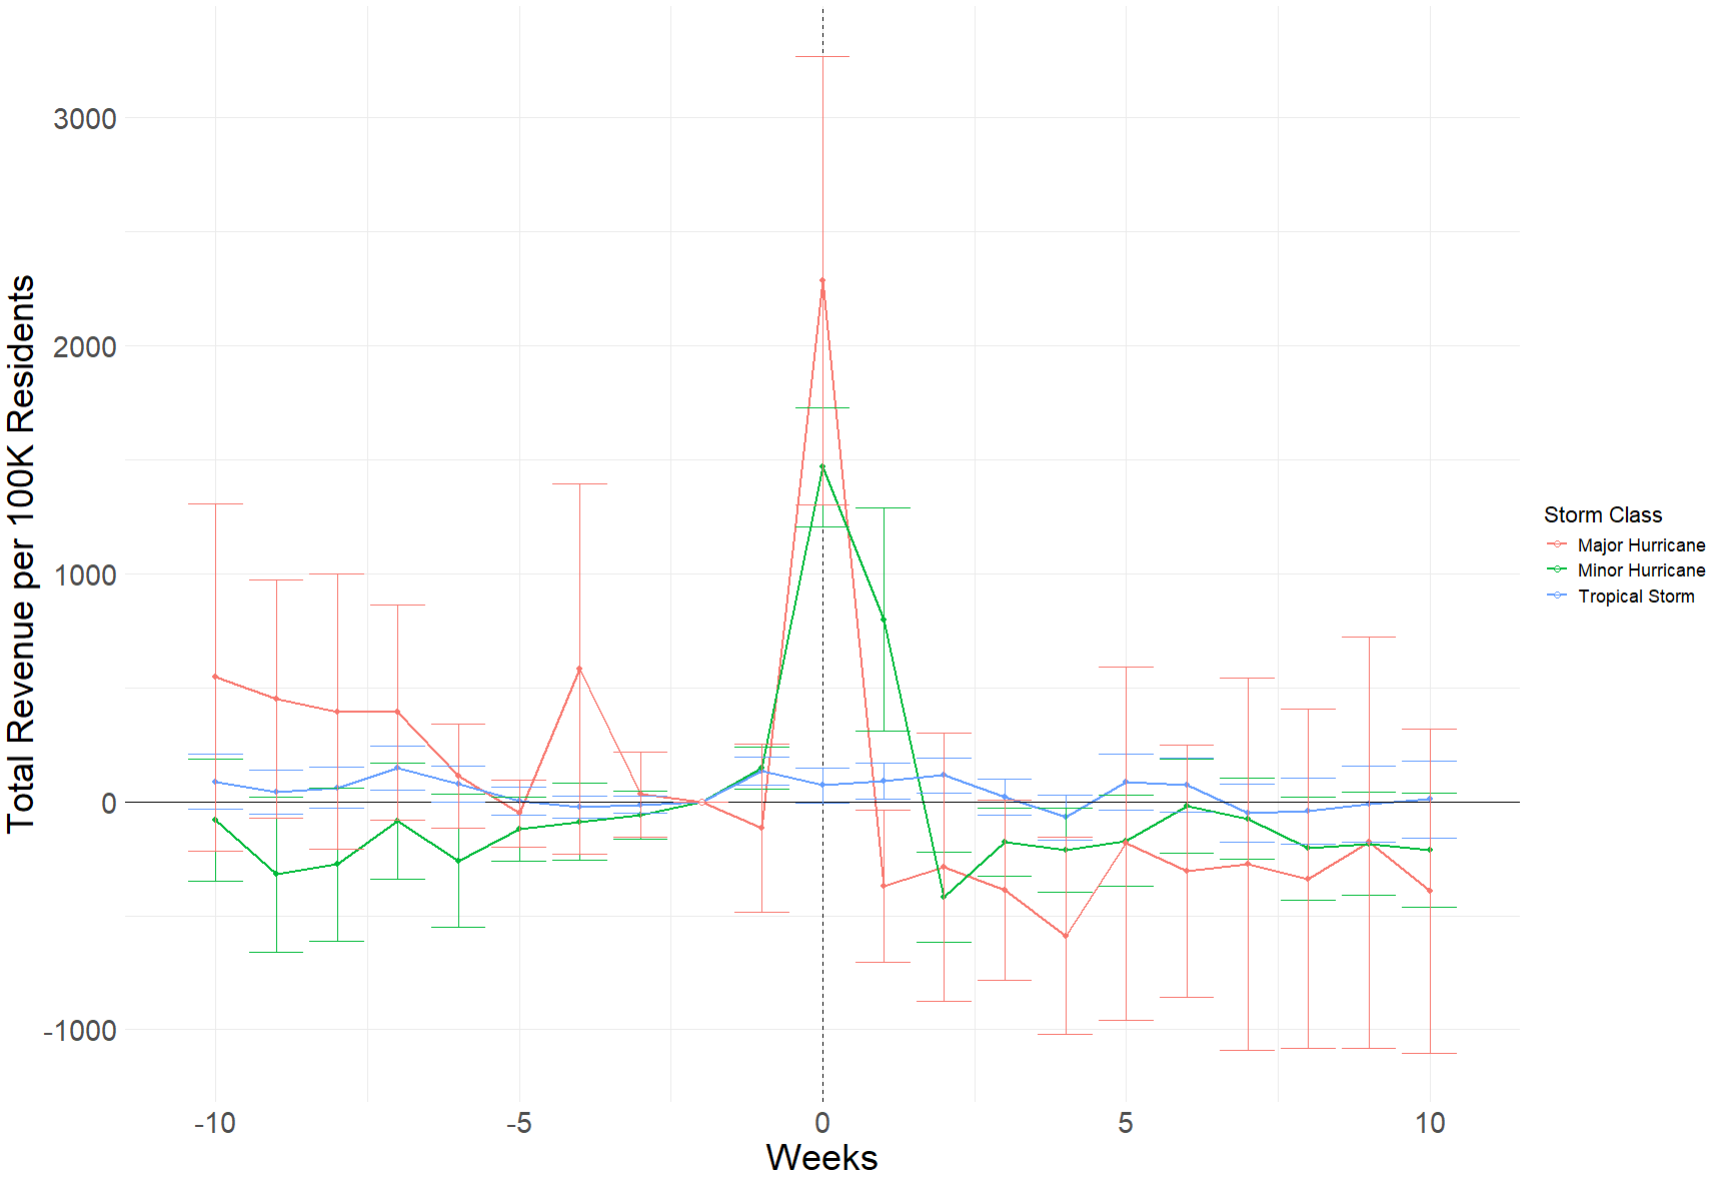
\includegraphics[width =0.7\linewidth]{ES type errors.png}
    \caption{Event Studies by Hurricane Category}
    \label{fig:type_ci}
    \floatfoot{Note: Results from event study with subsets based on hurricane category. The vertical axis represents total revenue per 100 thousand residents in USD. The horizontal axis represents weeks. Week 0 is the week that a tropical hurricane made landfall in a county. The bars around each point represents the 95\% confidence interval.}
\end{figure}


\begin{figure}[t!]
   \centering
	\begin{subfigure}{0.45\linewidth}
		\caption{1 to 4}
		
\includegraphics[width=\linewidth]{images/hist q1.png}
	\end{subfigure}
	\begin{subfigure}{0.45\linewidth}
		\caption{5 to 6}
		
\includegraphics[width=\linewidth]{images/hist q2.png}
	\end{subfigure}
		\begin{subfigure}{0.45\linewidth}
		\caption{7 to 8}
		
\includegraphics[width=\linewidth]{images/hist q3.png}
	\end{subfigure}
		\begin{subfigure}{0.45\linewidth}
		\caption{9 to 13}
		
\includegraphics[width=\linewidth]{images/hist q4.png}
	\end{subfigure}
  \caption{Event Study by Prior Landfall Count}
  \floatfoot{Note: Results from event study with subsets by landfall count from 1983 to 2007. The vertical axis represents total revenue per 100 thousand residents in USD. The horizontal axis represents weeks. Week 0 is the week that a tropical hurricane made landfall in a county. The ribbon around the point estimates represents the 95\% confidence interval.}
\label{fig:ES_hist_quant}
\end{figure}


\begin{figure}[h!]
    \centering
    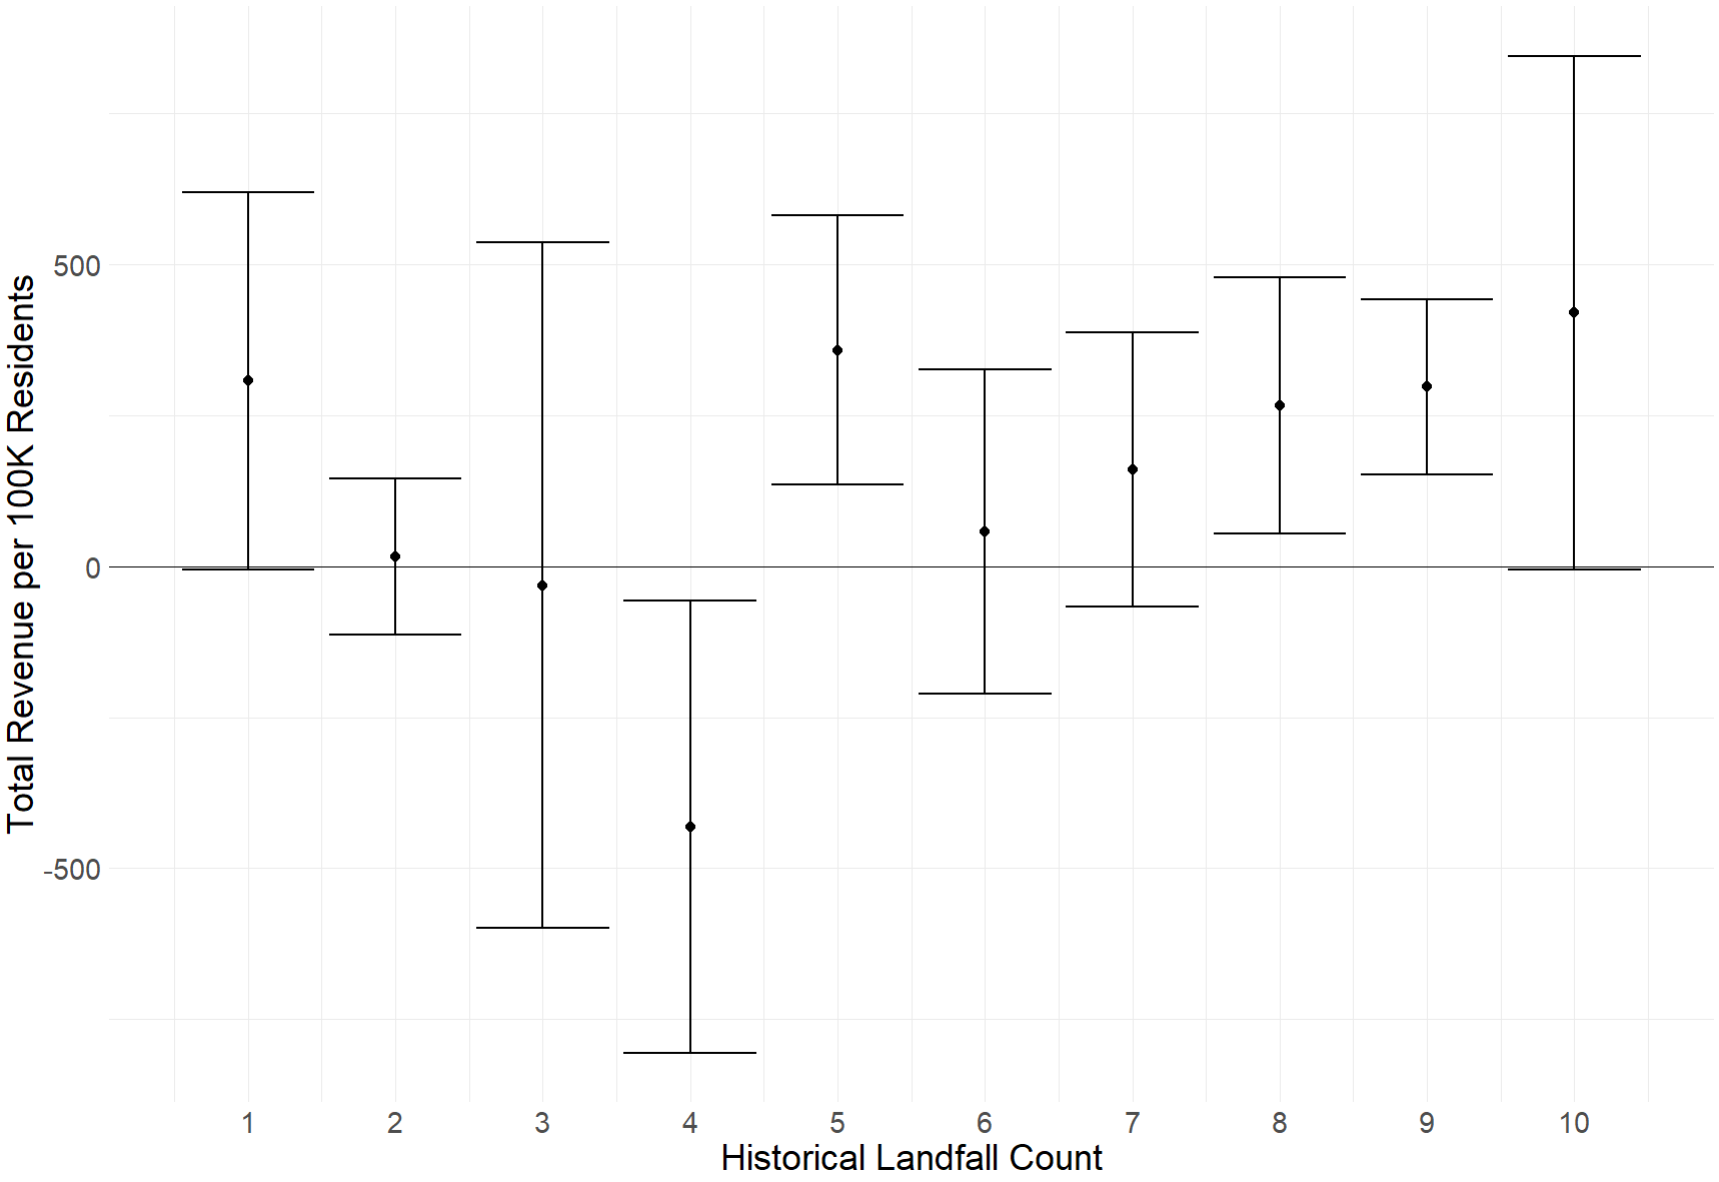
\includegraphics[width =0.7\linewidth]{ES past week 1.png}
    \caption{Event Study of Sales One Week Before Landfall}
    \label{fig:hist_before}
    \floatfoot{Note: Results from event study with subsets by hurricane landfall count from 1983 to 2007. The vertical axis represents total revenue per 100 thousand residents in USD. The horizontal axis represents weeks. The bars around each point represents the 95\% confidence interval.}
\end{figure}


\begin{figure}[h!]
    \centering
    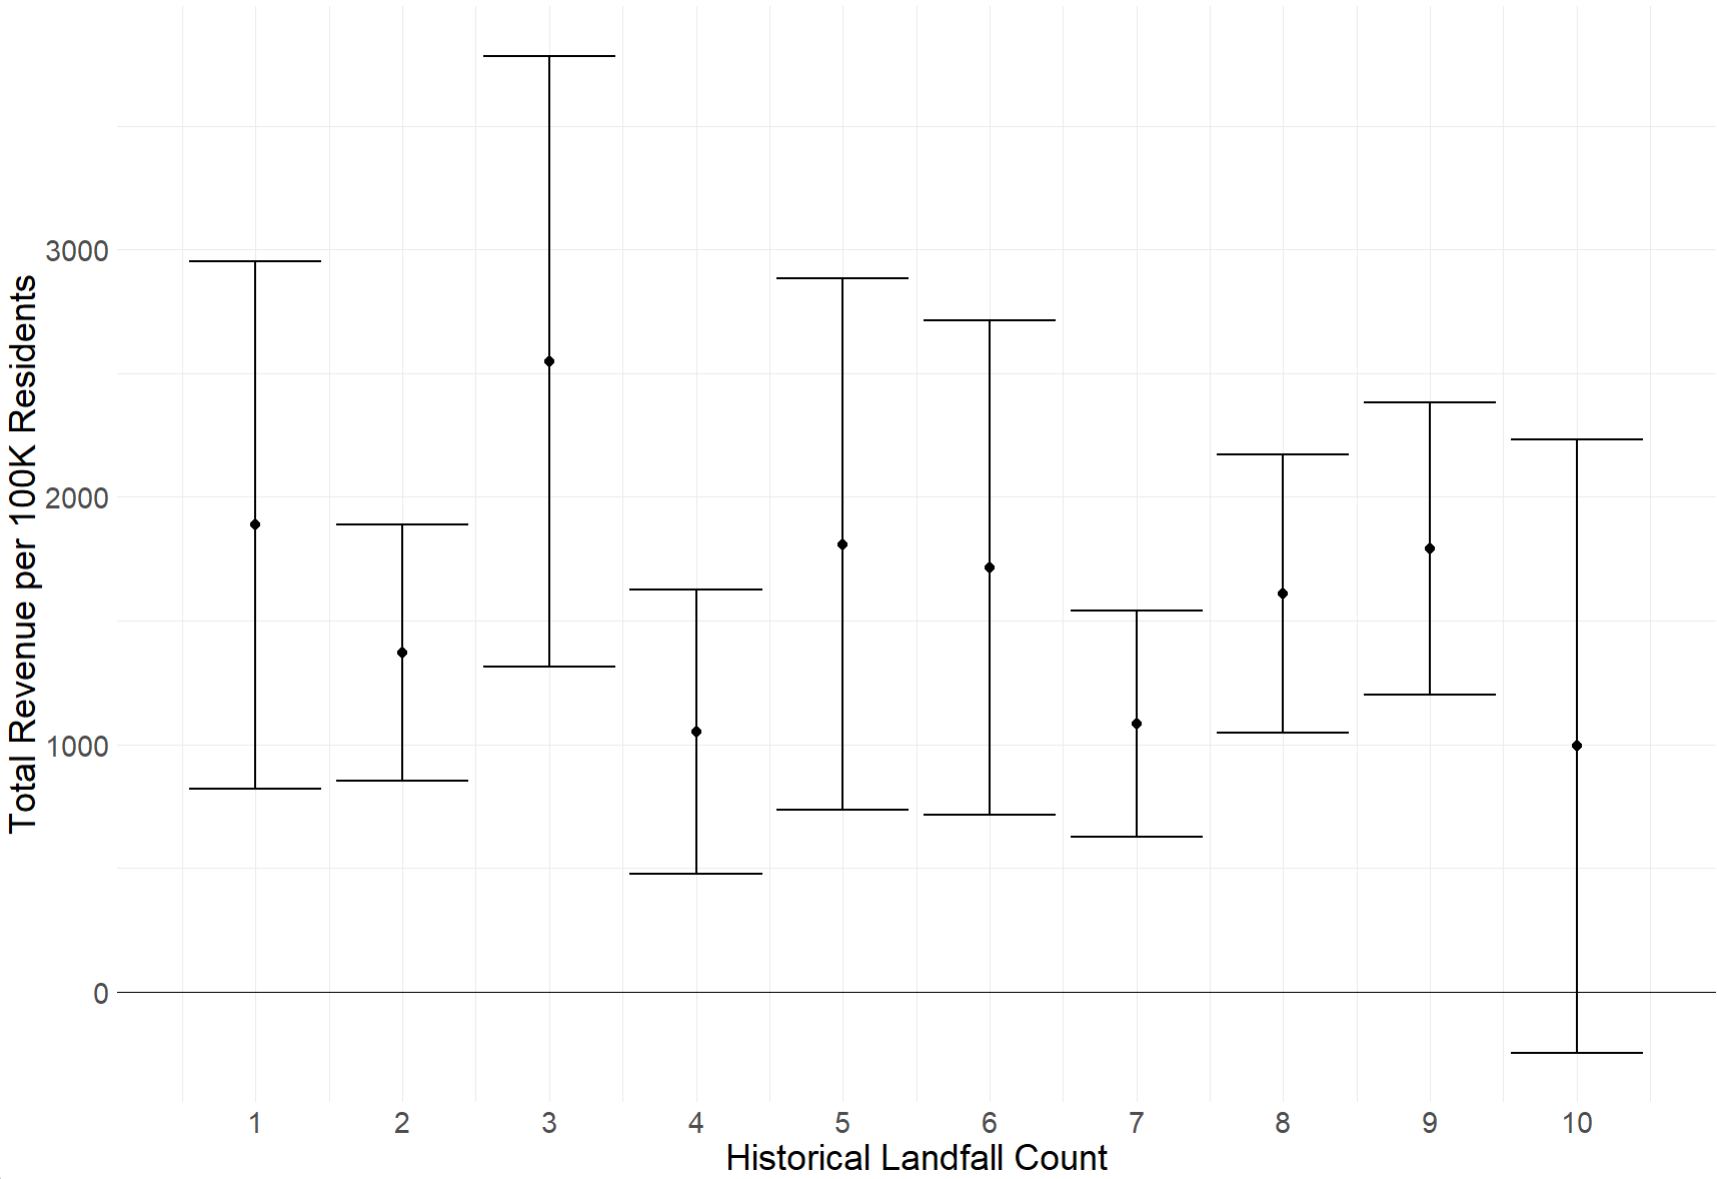
\includegraphics[width =0.7\linewidth]{ES hist week 0.png}
    \caption{Event Study of Sales the Week of Landfall}
    \label{fig:hist_during}
    \floatfoot{Note: Results from event study with subsets by hurricane landfall count from 1983 to 2007. The vertical axis represents total revenue per 100 thousand residents in USD. The horizontal axis represents weeks. The bars around each point represents the 95\% confidence interval.}
\end{figure}



\begin{table}[htbp]
   \caption{Recent Exposure Results}
   \centering
   \begin{tabular}{lcccc}
      \tabularnewline \midrule \midrule
      Dependent Variable: & \multicolumn{4}{c}{log(total\_rev\_per\_cap)}\\
      Model:                                   & (1)            & (2)            & (3)            & (4)\\  
      \midrule
      \emph{Variables}\\
      event                                    & 0.5645$^{***}$ & 0.5291$^{***}$ & 0.6481$^{***}$ & 0.7545$^{***}$\\   
                                               & (0.1143)       & (0.1164)       & (0.1444)       & (0.1812)\\   
      temp\_mean                               & 0.0045$^{***}$ & 0.0065$^{***}$ & 0.0065$^{***}$ & 0.0065$^{***}$\\   
                                               & (0.0010)       & (0.0010)       & (0.0010)       & (0.0009)\\   
      past\_25\_h1\_5                          &                & -0.0869$^{**}$ & -0.0869$^{**}$ & -0.0755$^{**}$\\   
                                               &                & (0.0345)       & (0.0345)       & (0.0330)\\   
      years\_since\_landfall                   &                & 0.0145$^{**}$  & 0.0146$^{**}$  & 0.0397$^{***}$\\   
                                               &                & (0.0065)       & (0.0065)       & (0.0101)\\   
      event $\times$ years\_since\_landfall    &                &                & -0.0156        & -0.0522$^{*}$\\   
                                               &                &                & (0.0089)       & (0.0277)\\   
      yrs\_since\_hur\_sq                      &                &                &                & -0.0014$^{**}$\\   
                                               &                &                &                & (0.0005)\\   
      event $\times$ yrs\_since\_hur\_sq       &                &                &                & 0.0018$^{*}$\\   
                                               &                &                &                & (0.0010)\\   
      \midrule
      \emph{Fixed-effects}\\
      fips                                     & Yes            & Yes            & Yes            & Yes\\  
      year                                     & Yes            & Yes            & Yes            & Yes\\  
      month                                    & Yes            & Yes            & Yes            & Yes\\  
      \midrule
      \emph{Fit statistics}\\
      Observations                             & 448,123        & 190,566        & 190,566        & 190,566\\  
      R$^2$                                    & 0.77146        & 0.79132        & 0.79134        & 0.79392\\  
      \midrule \midrule
      \multicolumn{5}{l}{\emph{Clustered (fips \& year) standard-errors in parentheses}}\\
      \multicolumn{5}{l}{\emph{Signif. Codes: ***: 0.01, **: 0.05, *: 0.1}}\\
   \end{tabular}
\end{table}


\begin{figure}[htbp]
    \centering
    % Embed the first page of the PDF as a scaled image
    \includegraphics[width=\textwidth, page=2]{ready-supply-kit-checklist.pdf}
    \caption{Emergency Supply Checklist from ``ready.gov''}
    \label{fig:checklist}
\end{figure}



\end{appendices}


\end{document}